\chapter{Validation, convergence and conservation experiments}
\chaptermark{Numerical experiments}
\label{cha:numer-experiments}

In this section we apply the various numerical methods constructed throughout this thesis to some micromagnetics problems.

The first case examined is a 2D problem without magnetostatics, where there is a known wave-like analytical solution for certain initial conditions.
This allows us to test the convergence of the various discretisations when applied to the LLG with exchange effective field.
It also allows us to test the geometric integration properties of the IMR.

The second problem is another simple case, but with no analytical solution: a non-uniform applied field is used to induce non-uniform dynamics in a 2D problem without magnetostatics.
This allows us to test geometric integration properties of the IMR in the absence of an analytical solution.

We then show results from the \mumag standard problem \#4 \cite{mumag-website}, which is widely used to test dynamic micromagnetic codes.
This allows us to verify the complete model and to examine the geometric integration properties when the FEM/BEM magnetostatics calculations are included.


\section{Example with a wave-like solution}
\label{sec:numer-exper}

\subsection{Problem definition}
\label{sec:wave-problem-definition}

In this experiment we solve a micromagnetic problem which has a wave-like exact solution in 2D, the details of this solution are given in \cref{sec:wave-like-solution}.
We solve the LLG without magnetostatics on a two dimensional square domain $\magd = [0,1] \times [0,1]$ with periodic boundary conditions.
We integrate time over $T = [0, 5]$.
This solution is obtained by setting the initial condition according to \cref{eq:97}:
\begin{equation}
  \begin{aligned}
    m_x(0) &= \sin(c) \cos\bigb{\kvec \cdot \xv}, \\
    m_y(0) &= \sin(c) \sin\bigb{\kvec \cdot \xv}, \\
    m_z(0) &= \cos(c),
  \end{aligned}
\end{equation}
and using $\happ = \zerov$.
The solution parameters used are $\kvec = 2\pi$ (so that the solution is periodic on domains of unit size), $c = 0.1\pi$, and $\dampc = 0.01$.
For the energy conservation experiments $\dampc = 0$ is used instead.

This problem allows us to examine the convergence and geometric integration properties of IMR with the FEM using nodal quadrature.
In particular the existence of an exact solution allows us to easily measure the convergence rate for the various methods.
This allows us to explore the effects of the geometric integration properties of IMR on the solution accuracy.


\subsection{Implementation details}
\label{sec:impl-deta}

We use the finite element method as discussed in \cref{sec:galerk-meth-llg} to spatially discretise the LLG equation.
Unless otherwise specified we use a mesh of square elements with $5 \times 2^4$ elements along each edge.
For the evaluation of the resulting integrals both the nodal quadrature discussed in \cref{sec:local-nodal-integr} and standard Gaussian quadrature methods are used.

For time integration the adaptive IMR, TR and BDF2 methods are used with a tolerance of $\toltt = 10^{-5}$ and an initial time step of $\dtx{0} = 10^{-5}$ (significantly smaller than the time step selected by an initial experimental run).
The methods which do not naturally conserve $\abs{\mv}$ (TR and BDF2 methods, and IMR with Gaussian quadrature is used) are run both with and without re-normalisation of the magnetisation.
The re-normalisation process is implemented by setting each nodal value of the magnetisation to $\mv_i = \mv_i/\abs{\mv_i}$ after each time step (after the selection of the next step size to avoid complicating the adaptivity process).

Linearisation is handled using the Newton-Raphson method with Newton tolerance set to $\ntol = 10^{-12}$ (unless otherwise specified).
The resulting linear systems are solved using GMRES with an ILU(1) preconditioner as described in \cref{sec:llg-only-system}.

The adaptive IMR integrator, as described in \cref{sec:adaptive-imr}, requires the computation of an explicit time step.
For this step we use the Landau-Lifshitz form of the LLG discretised in exactly the same way as described in \cref{sec:galerk-meth-llg}.
The resulting linear system (involving only a mass matrix) is solved using the method of conjugate gradients preconditioned by the lumped mass matrix (\ie the diagonal matrix of the row sums).
Note that when nodal quadrature is used the mass matrix is a diagonal matrix and no linear solve is needed (see \cref{sec:nodal-integration}).


\subsection{General results}

An example snapshot of the solution at time $t=0.1$ is shown in \cref{fig:2d-wave-snapshot}.
Over time the wave moves in the $[-1,-1]$ direction and is simultaneously damped out towards the $\mv = [0,0,1]$ state.

\begin{figure}
  \centering
  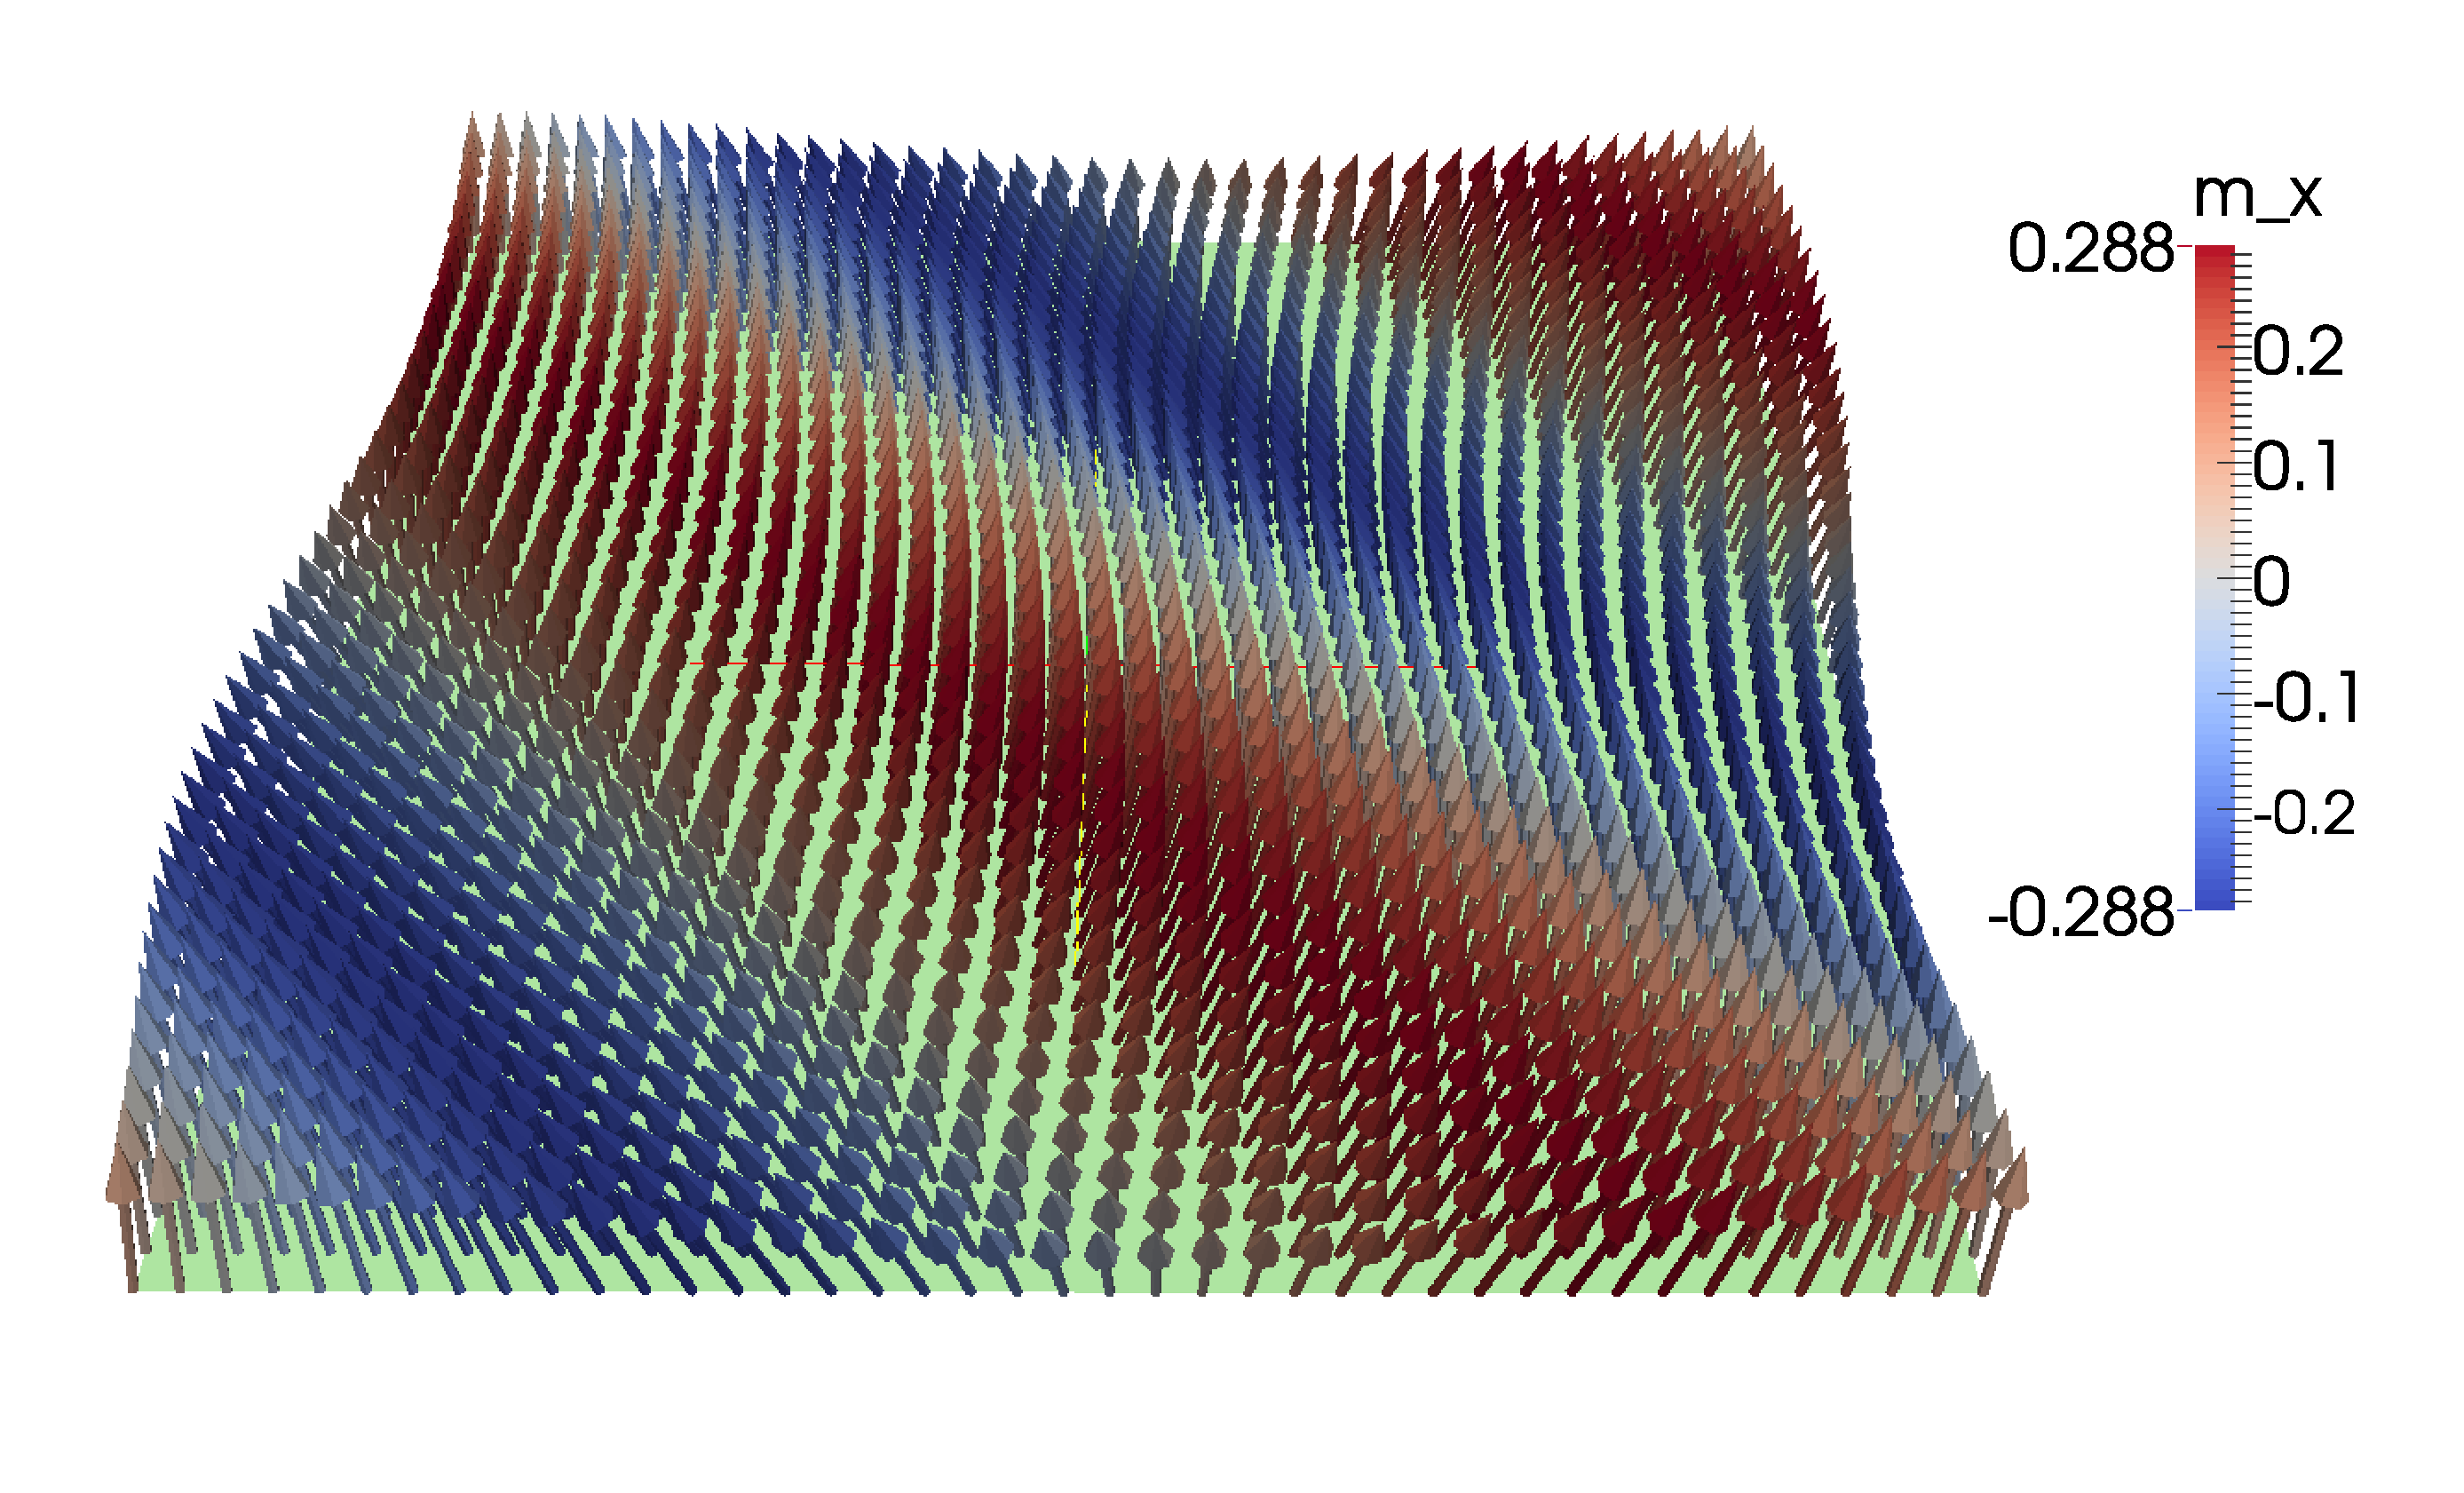
\includegraphics[width=0.8\textwidth]{images/2d_wave_picture_t0p1.pdf}
  \caption{Snapshot of the approximate solution for the 2D wave problem at $t=0.1$ time units obtained using adaptive IMR with nodal integration.
    Colour indicates the value of $m_x$.
    The $z$-component of the magnetisation is constant over the domain with $m_z = 0.958$.}
  \label{fig:2d-wave-snapshot}
\end{figure}

The behaviour of the approximate solutions over time at $\xv = \zerov$ is shown in \cref{fig:2d-wave-time-trace}.
Only results from the methods without re-normalisation are shown because they are identical to the equivalent method with re-normalisation (where applicable) at the scale of the plot.

The time steps selected by the various algorithms for this problem are also shown in \cref{fig:2d-wave-time-trace}.
The appearance of a jump in the time step size at $t=0$ is due to the algorithms rapidly increasing the time step size from the small initial value to a step size appropriate for the given tolerance.
After an appropriate step size is reached there is a smooth, gradual increase as the solution is damped out.
This is as expected, in particular note that there is no oscillation of the step size with the precessional motion as was observed in \cref{sec:aimr-llgode-numerical-results}.

\begin{figure}
  \centering
  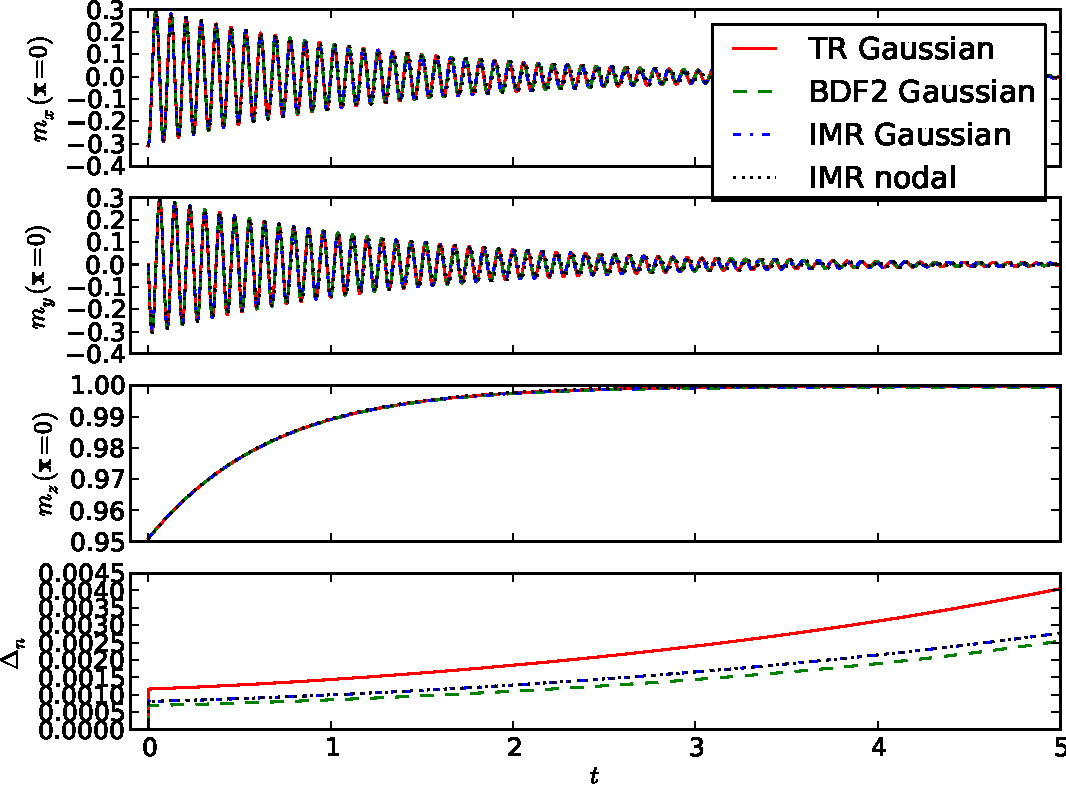
\includegraphics[width=0.9\textwidth]{plots/2d_wave_solution_time_trace/get2oftracevaluesvs-get3oftracevaluesvs-get4oftracevaluesvs-dtsvstimes.pdf}
  \caption{The temporal behaviour of the wave solution at $\xv = \zerov$ and the time step selected by the various adaptive integration schemes without re-normalisation.
    }
  \label{fig:2d-wave-time-trace}
\end{figure}


\subsection{Convergence study}

Since we have an exact solution for this example we can easily calculate an error norm and plot the convergence as both the time step $\dtn$ and the element edge length $h$ go to zero.
Following the example of Jeong \etal \cite{Jeong2014} we link the time step size to the spatial discretisation size by $\dtn = 0.32h$.
It is important to note that, in contrast to explicit time integration schemes, this coupling of the time and space discretisation parameters is \emph{not} required for stability, it is merely more convenient to experiment with a single parameter than with two independent parameters.
We choose element edge lengths of $h = 1/(5 \cdot 2^n)$ with $n=1,2,3,4,5,6$.
% Larger values of $n$ grow extremely computationally expensive for two reasons: firstly because we choose to reduce the time step and $h$ simultaneously, and so require more solves of larger systems.
% Secondly our iterative linear solver becomes less effective due to the extremely large systems involved ($\sim 10^6$ rows with $n=8$).

In these experiments we always use re-normalisation for schemes which are not expected to naturally conserve $\abs{\mv}$ because in practical applications such schemes would not be used without re-normalisation.

As a first convergence experiment we examine the norm of the error after a single time step
\begin{equation}
  \merr_{,1} = \norm{\mv(\xv_j, t_1) - \mv_{j,1}}_2.
\end{equation}
In this case we expect the convergence (in both space and time) to be second order for all methods.
The results of this experiment are shown in \cref{fig:convergence-one-step},
We see that convergence is indeed second order for all methods and that the accuracy for the BDF2 scheme is a worse than the other schemes by a roughly constant factor.
We also see that the use of nodal quadrature results in an error increase by a small constant factor.
This indicates that the geometric integration properties of IMR with nodal quadrature give no benefit for a single time step, as would be expected.
\begin{figure}
  \centering
  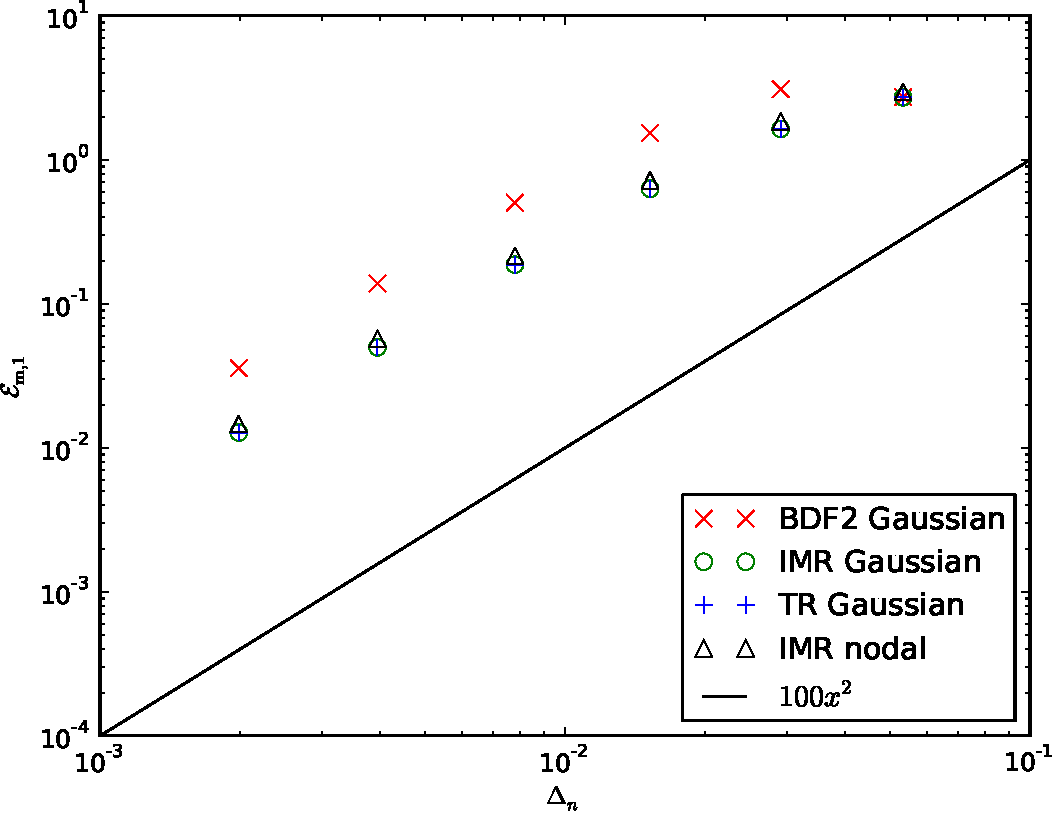
\includegraphics[width=0.9\textwidth]{plots/2d_wave_solution_convergence_long_time/firstoferrornormsvsfakemeanofdts.pdf}
  \caption{Convergence in the error norm $\errmpde{}$ after a single step of time integration for the 2D wave-like problem.}
  \label{fig:convergence-one-step}
\end{figure}



We also wish to examine a norm of the error after a large number of time steps, so for the rest of the experiments in this section we examine the integral of the error norm over $T = [0, 5]$.
However, reaching the levels of convergence required for $\errmpde$ to be meaningful is difficult because the ``worst case'' for the norm is that the approximated magnetisation is out of phase with the exact solution (\ie the error norm is bounded).
A plot of the time integral of $\errmpde$ is shown in \cref{fig:convergence-long-time-full-norm}, as expected no convergence is seen until the spatial/temporal refinement level reaches $n=5$ for IMR and TR, and not at all for BDF2.
\begin{figure}
  \centering
  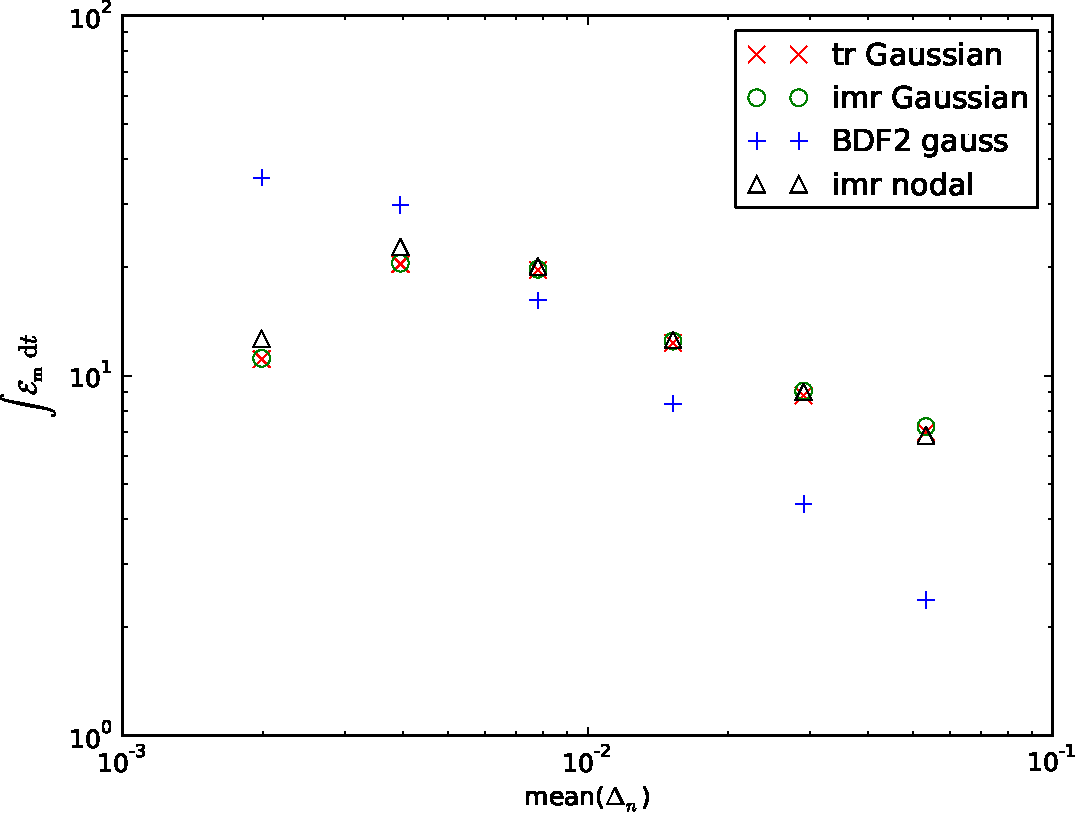
\includegraphics[width=0.9\textwidth]{plots/2d_wave_solution_convergence_long_time/errornormintegralvsmeanofdts.pdf}
  \caption{Convergence of $\intt{\errmpde}$, where $T=[0,5]$, for the 2D wave-like problem.
  }
  \label{fig:convergence-long-time-full-norm}
\end{figure}

To obtain more meaningful results we should use an alternative error norm which allows a better measure of the error even for approximate solutions which are out of phase with the exact solution.
One such error norm measures the deviation of $m_z$ from the exact value
\begin{equation}
  \errmz = \max_j \abs{m_{z,j,k} - m_z(t_n)}.
\end{equation}
Note that the exact value of $m_z$ is not a function of $\xv$ and so it is sufficient to take the maximum value.
This error norm measures the level of over/under damping caused by the approximation.

The convergence results for the time integral of the error norm $\errmz$ are shown in \cref{fig:convergence-long-time-mz-norm}.
We again see second order convergence behaviour for all methods.
The BDF2 method requires additional refinement to reach the asymptotic convergence behaviour, and has around an order of magnitude larger error than the other methods once convergence is reached.
Also note that there is no significant difference between IMR with nodal quadrature (which conserves $\abs{\mv}$) and IMR with Gaussian quadrature (in which $\mv$ is re-normalised), indicating that geometric integration offers no significant benefits in this case.
\begin{figure}
  \centering
  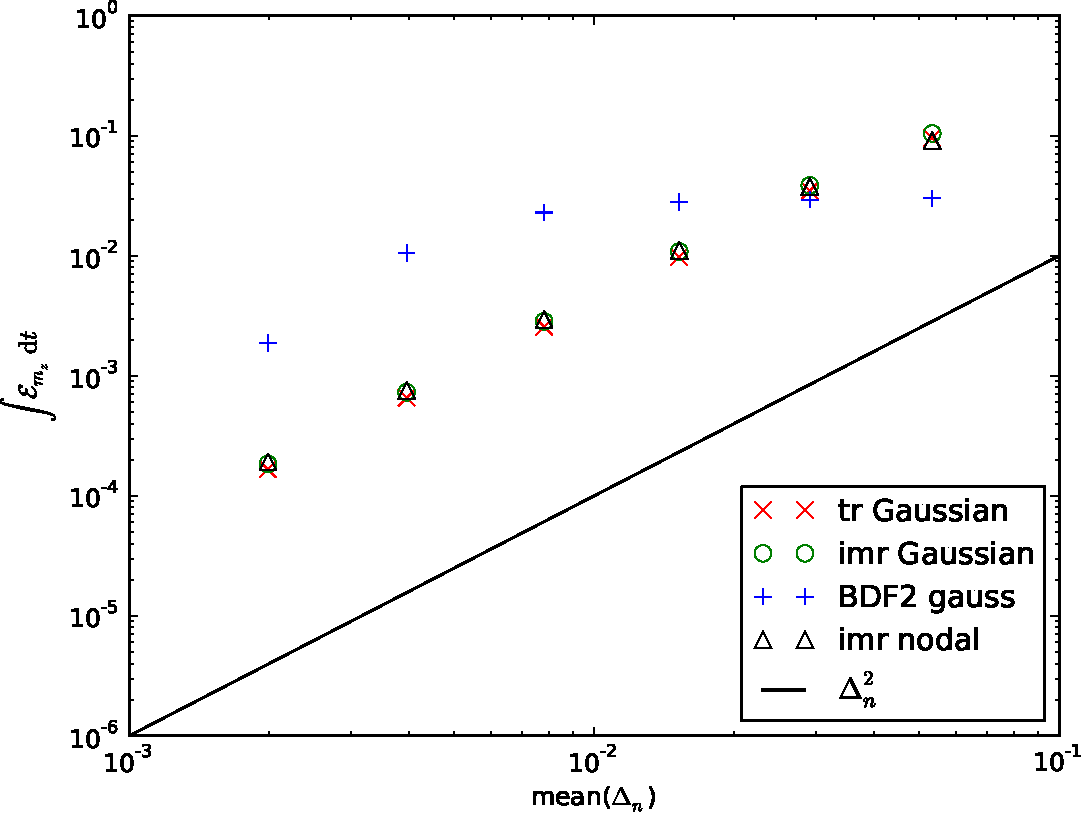
\includegraphics[width=0.9\textwidth]{plots/2d_wave_solution_convergence_long_time/auxerr1integralvsmeanofdts.pdf}
  \caption{Convergence of $\intt{\errmz}$, where $T=[0,5]$, for the 2D wave-like problem.
  }
  \label{fig:convergence-long-time-mz-norm}
\end{figure}

% % fix or remove:
% Our next error norm aims to measure the error in the frequency of the wave.
% It is defined as
% \begin{equation}
%   \begin{aligned}
%     \errphase &= \abs{\psi_{n,0} - \psi(t_n, 0)}, \\
%     &= ...,
%   \end{aligned}
% \end{equation}
% where $\psi(t_n, 0) = ...$ is the analytical phase of the wave at $\xv = \zerov$, and $\psi_{n,0}$ is the corresponding phase in approximate solution.
% The convergence results with this error norm are shown in \cref{fig:convergence-long-time-phase-norm}.
% Unfortunately it appears that this error norm is not much better than $\errmpde$ in terms of measuring the error outside of the asymptotic regime, and we can only draw the same conclusions as for that example.
% \begin{figure}
%   \centering
%   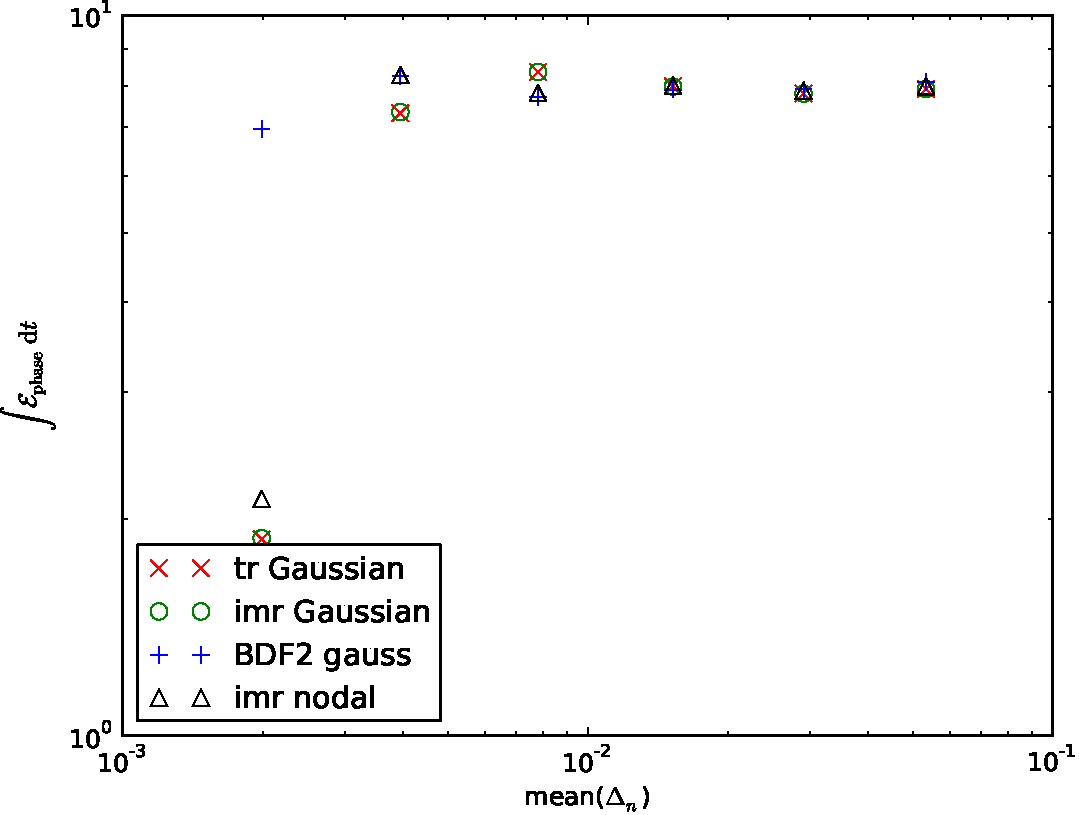
\includegraphics[width=0.9\textwidth]{plots/2d_wave_solution_convergence_long_time/auxerr0integralvsmeanofdts.pdf}
%   \caption{Convergence of $\intt{\errphase}$, where $T=[0,5]$, for the 2D wave-like problem.
%   }
%   \label{fig:convergence-long-time-phase-norm}
% \end{figure}



\subsection{Geometric integration properties}
\label{sec:2d-wave-results-cons-prop}

We now examine the error in nodal magnetisation length:
\begin{equation}
  \myerr_{\abs{\mv}}(t_n) = \max_j \abs{\abs{\mv_{j,n}} - 1},
  \label{eq:102}
\end{equation}
in the approximations generated by each of the time integration schemes (without re-normalisation).
\Cref{fig:mean-ml-error-2d} shows the evolution of the maximum of \cref{eq:102} (over all nodes).
When using IMR with nodal quadrature the magnetisation length error remains extremely small, but for other methods the error rapidly grows to around $\order{10^{-4}}$ and seems to saturate at this level.
\begin{figure}
  \centering
  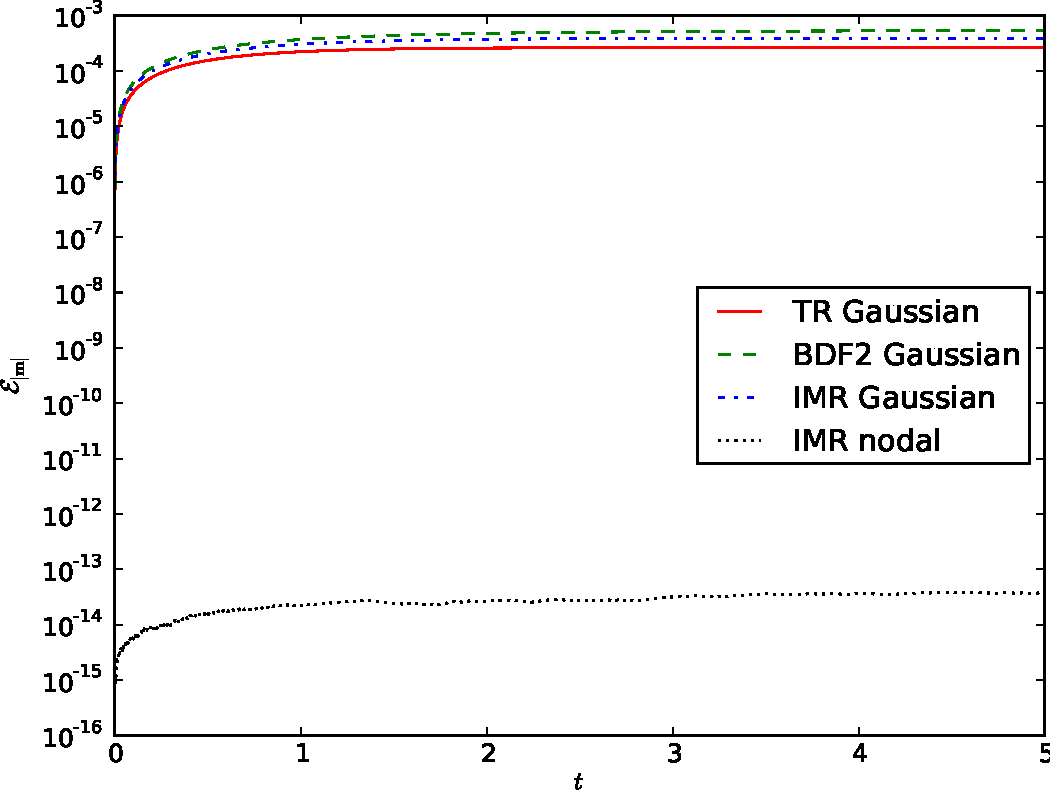
\includegraphics[width=0.8\textwidth]
  {plots/2d_wave_solution_m_length/mlengtherrormaxesvstimes.pdf}
  \caption{Evolution of $\myerr_{\abs{\mv}}$ with various time integrators and quadratures for the 2D wave-like problem.
  }
  \label{fig:mean-ml-error-2d}
\end{figure}

We next examine the energy conservation properties of the various schemes for the wave solution with $\dampc = 0$.
The only energy involved is the exchange energy, which can be calculated using \cref{eq:nd-e-ex}.
Note that these integrals can be evaluated exactly by any quadrature because $\grad \mv$ is a constant inside each element.
The results are shown in \cref{fig:energy-error-2d}, interestingly we see that IMR with Gaussian quadrature and TR both conserve energy in a similar manner to IMR with nodal quadrature.
This is likely due to some special property of the exact solution, and does not appear to be the case in general (see \cref{sec:non-uniform-applied}).
\begin{figure}
  \centering
  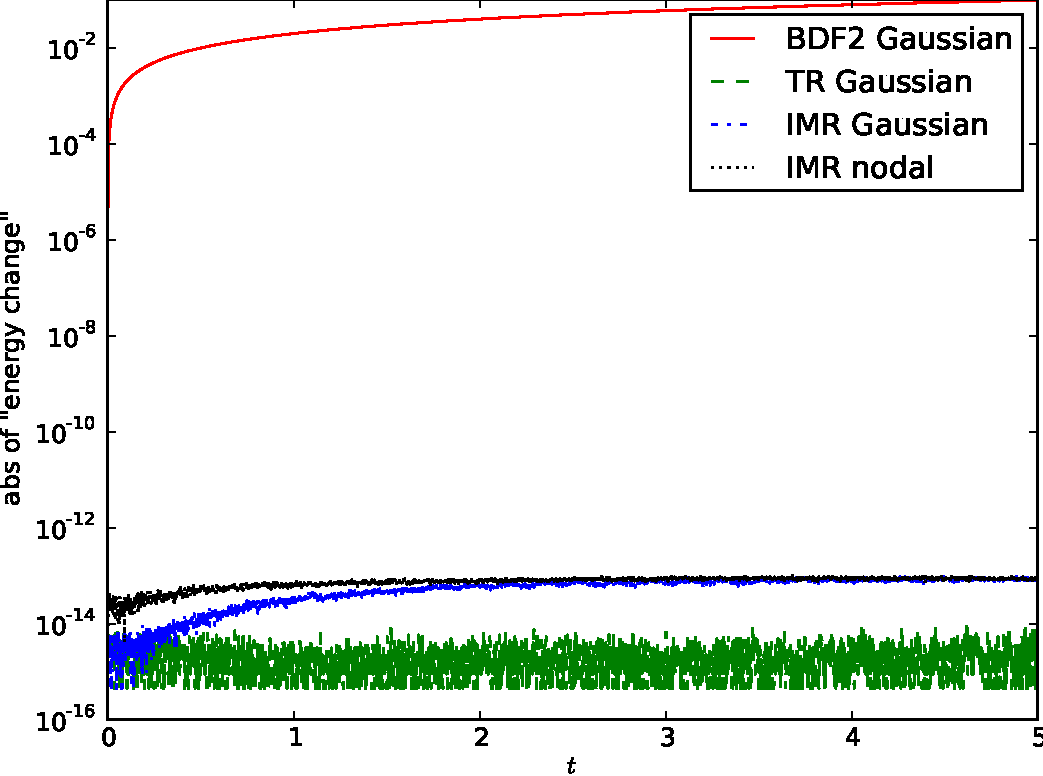
\includegraphics[width=0.8\textwidth]{plots/2d_wave_solution_energy/absofenergychangevstimes}
  \caption{Evolution of the error in energy with various time integration schemes and quadratures for the undamped 2D wave-like problem.
}
  \label{fig:energy-error-2d}
\end{figure}


\subsection{Effect of Newton tolerance}
\label{sec:effect-newt-toler-m-conservation}

As mentioned in \cref{sec:nodal-integration} we would expect to see some effect on the conservation properties when the accuracy of the linearisation method is varied.
In our implementation the Newton-Raphson method is used for linearisation, so the relevant measure of accuracy is the Newton tolerance, $\ntol$.

The obvious experiment to carry out would be to vary the Newton tolerance and examine how the error in $\abs{\mv}$ is affected.
However the Newton-Raphson method converges extremely quickly meaning that the final residual is often many orders of magnitude smaller than the tolerance, this would hide any correlation between the tolerance and the error.
Instead we plot the error against the \emph{actual} converged residual norm (specifically: the mean over all time steps of $\norm{\rv}_\infty$ after the Newton method has converged for that time step).
In order to generate a variety of converged residual norms we run the experiment with a range of parameters: $\ntol = 10^{-8}, 10^{-9}, 10^{-10}, 10^{-11}, 10^{-12}$; $\toltt = 10^{-3}, 10^{-4}, 10^{-5}$; $\dampc = 1, 0.001, 0$; and $h = 0.05, 0.025, 0.0125$.
We only integrate in time over the shorter interval $T = [0, 1]$ due to the volume of computations required.
The results are shown in \cref{fig:ml-error-2d-nodal-newton-tests}, there is a clear correlation between the magnitudes of the final residuals and the error in $\abs{\mv}$.
A similar result is seen in \cref{fig:energy-error-2d-nodal-newton-tests} for the energy conservation property when $\dampc = 0$.

\begin{figure}
  \centering
  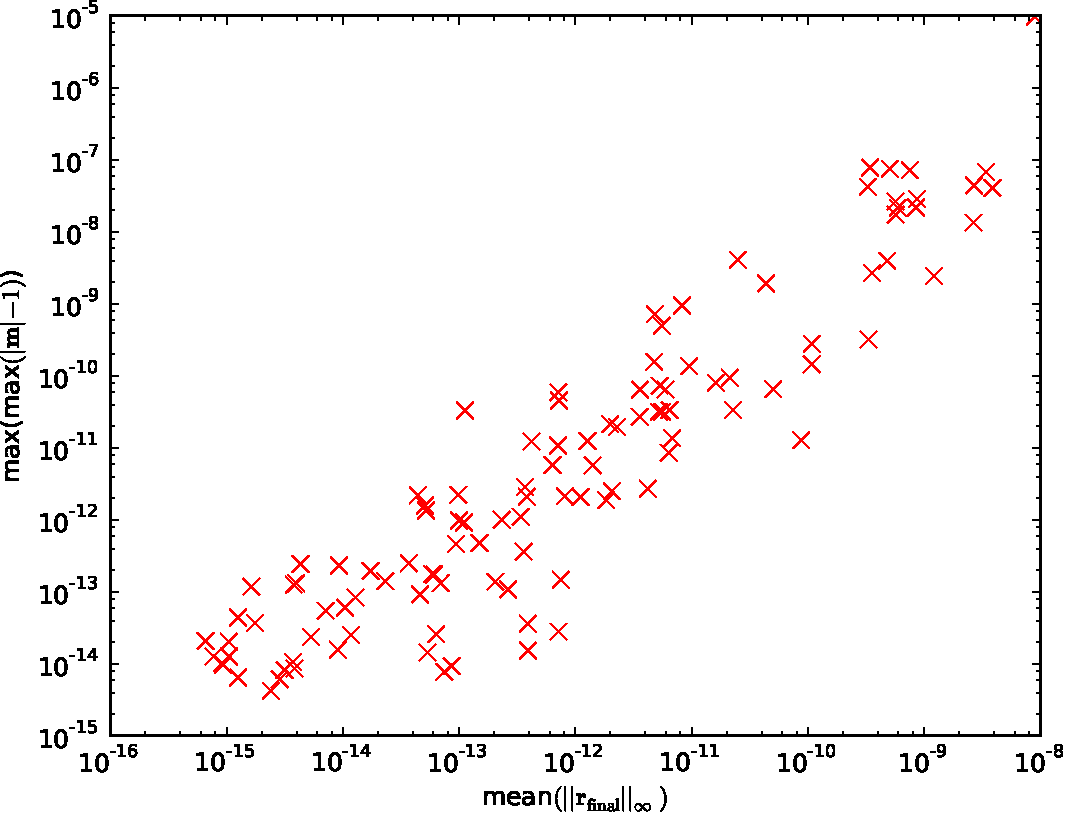
\includegraphics[width=0.8\textwidth]
{plots/2d_wave_solution_m_length_newton_res/maxofmlengtherrormaxesvsmeanminofnewtonresiduals.pdf}
  \caption{Correlation between maximum (over all nodes and all time steps) error of nodal magnetisation lengths and the mean (over time) of the converged Newton residual norm in the 2D wave-like problem solved using adaptive IMR and nodal quadrature.
  }
  \label{fig:ml-error-2d-nodal-newton-tests}
\end{figure}


\begin{figure}
  \centering
  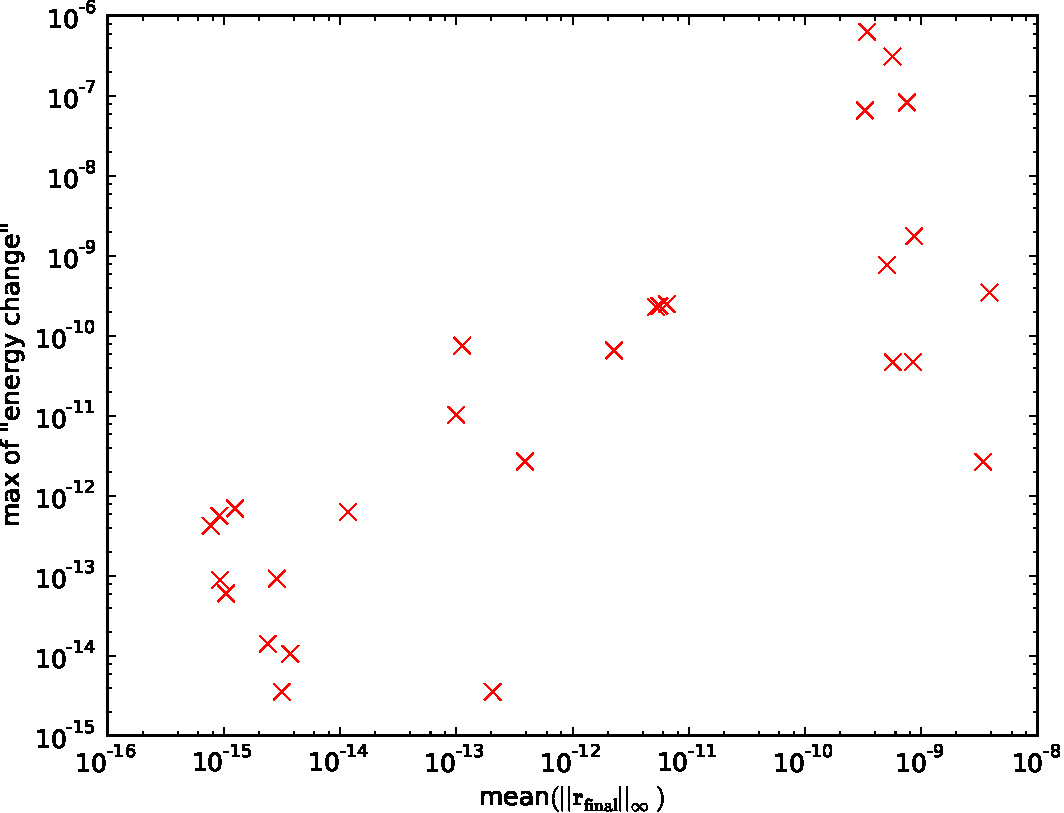
\includegraphics[width=0.8\textwidth]
  {plots/2d_wave_solution_energy_newton_res/maxofenergychangevsmeanminofnewtonresiduals.pdf}
  \caption{Correlation between the maximum (over time) of the error in energy and the mean (over time) of the converged Newton residual norm in the undamped 2D wave-like problem solved using adaptive IMR and nodal quadrature.
  }
  \label{fig:energy-error-2d-nodal-newton-tests}
\end{figure}



\subsection{Conclusions}

We have shown that the methods we tested have the expected convergence and time step selection properties.
We also observed that the asymptotic accuracy of the BDF2 method is lower than the TR or IMR methods by a moderately sized constant factor.

We have also shown that the geometric integration properties of IMR are preserved in a weak form FEM model when used with a nodal quadrature scheme.
Finally we have shown that these properties are linked to the accuracy of the non-linear solver, as predicted in \cref{sec:nodal-integration}.

We have also observed unexpected geometric integration properties when IMR with Gaussian quadrature or TR are used.
It is expected that this is a consequence of the specific test problem rather than the methods themselves.
This conjecture will be tested in the next section.

Since all time integration schemes except for BDF2 showed some geometric integration properties the effect of such properties on the overall error cannot be analysed using this example.


\FloatBarrier
\section{An example with non-uniform applied field}
\label{sec:non-uniform-applied}

In \thisref{sec:non-uniform-applied} we construct a problem which is non-uniform in space without the involvement of the magnetostatic field by applying a non-uniform applied field.
This will allow us to examine whether the anomalous geometric integration properties observed in the previous section are related to the analytical solution.

This experiment also reveals some odd behaviour on meshes of triangular elements.

\subsection{Problem definition}

We solve the LLG without magnetostatics on a two dimensional square domain $\magd = [0,5] \times [0,5]$ with Neumann boundary conditions.
The problem is integrated in time over $T = [0, 5]$.

We use a uniform initial condition $\mv = [1, 1, 0]/\sqrt{2}$ with a non-uniform applied field
\begin{equation}
  \happ =
  \begin{cases}
    1.1 (1 -  x) & x  < 1, \\
    0 & \mathrm{otherwise}.
  \end{cases}
\end{equation}
As before we use $\dampc = 0.01$ except for energy conservation experiments where we use $\dampc = 0$.
The implementation details of this example are exactly as described in \cref{sec:impl-deta}, except that we also use meshes of triangular elements.
The structure of the triangular element mesh is equivalent to the square element case except with element is divided in diagonally into two triangles.

The dynamics occurring in this problem are quite simple: the magnetisation in the region of the domain $x<1$ moves towards $\mv = [0, 0, 1]$ by the applied field.
Exchange interactions force the rest of the domain to move towards the same field, albeit much more slowly, until eventually the entire domain is in a uniform state.


\subsection{Geometric Integration properties}


The evolution of the magnetisation length for this experiment is shown in \cref{fig:nonuniform-h-ml-error}, we see that in this case only IMR with nodal quadrature conserves $\abs{\mv}$ as expected.
The same is true for the energy conservation with zero damping, as shown in \cref{fig:nonuniform-h-energy-error}.

\begin{figure}
  \centering
  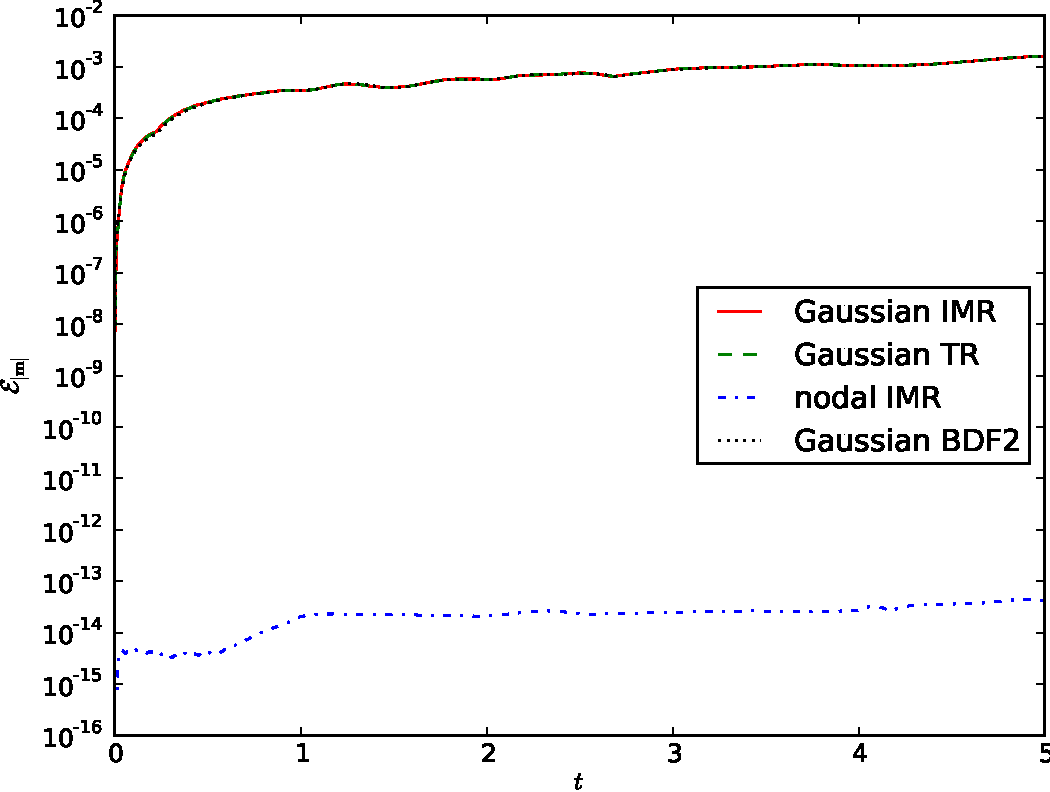
\includegraphics[width=0.8\textwidth]
  {plots/nonuniform-h-ml/mlengtherrormaxesvstimes.pdf}
  \caption{
    Evolution of $\myerr_{\abs{\mv}}$
    with various time integration schemes and quadratures
    for the 2D nonuniform field problem.
  }
  \label{fig:nonuniform-h-ml-error}
\end{figure}


\begin{figure}
  \centering
  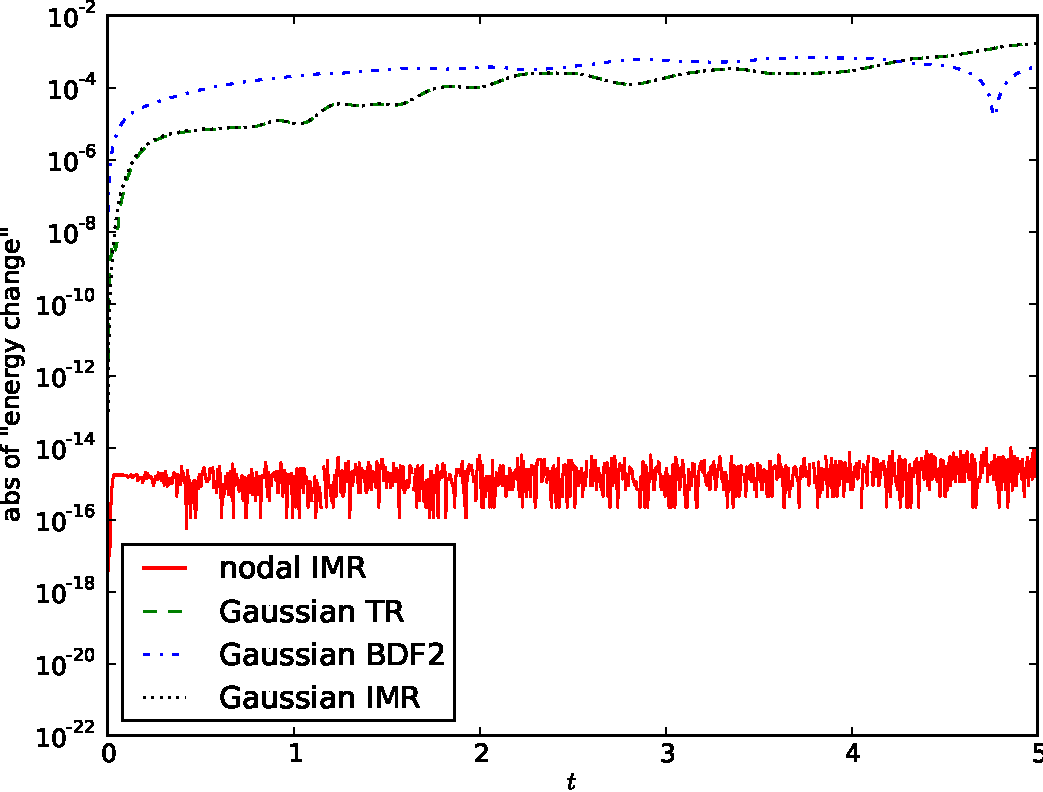
\includegraphics[width=0.8\textwidth]
  {plots/nonuniform-h-energy-change/absofenergychangevstimes.pdf}
  \caption{
    Evolution of the error in energy
    with various time integration schemes and quadratures
    for the undamped 2D nonuniform field problem.
  }
  \label{fig:nonuniform-h-energy-error}
\end{figure}


\subsection{Triangular meshes}
\label{sec:triangular-meshes}

Finally we show some anomalous results when a mesh of triangular elements is used.
The evolution of $\abs{\mv}$ is shown in \cref{fig:ml-error-triangle-mesh}.
We see that the $\abs{\mv}$ conservation property of IMR with nodal quadrature fails on triangular elements.
Similarly the conservation of energy (with $\dampc = 0$) fails, as shown in \cref{fig:energy-error-triangle-mesh}.
Other experiments show this issue for a variety of other cases including 3D problems with tetrahedral elements, but not for the wave-like example above.

We do not have an explanation for this effect.
However it should be noted that the non-conservation effects are small enough that they would not be noticed if the numerical experiments were run with a loose non-linear solver tolerance, such as used in \eg \cite{Bartels2006}.

\begin{figure}
  \centering
  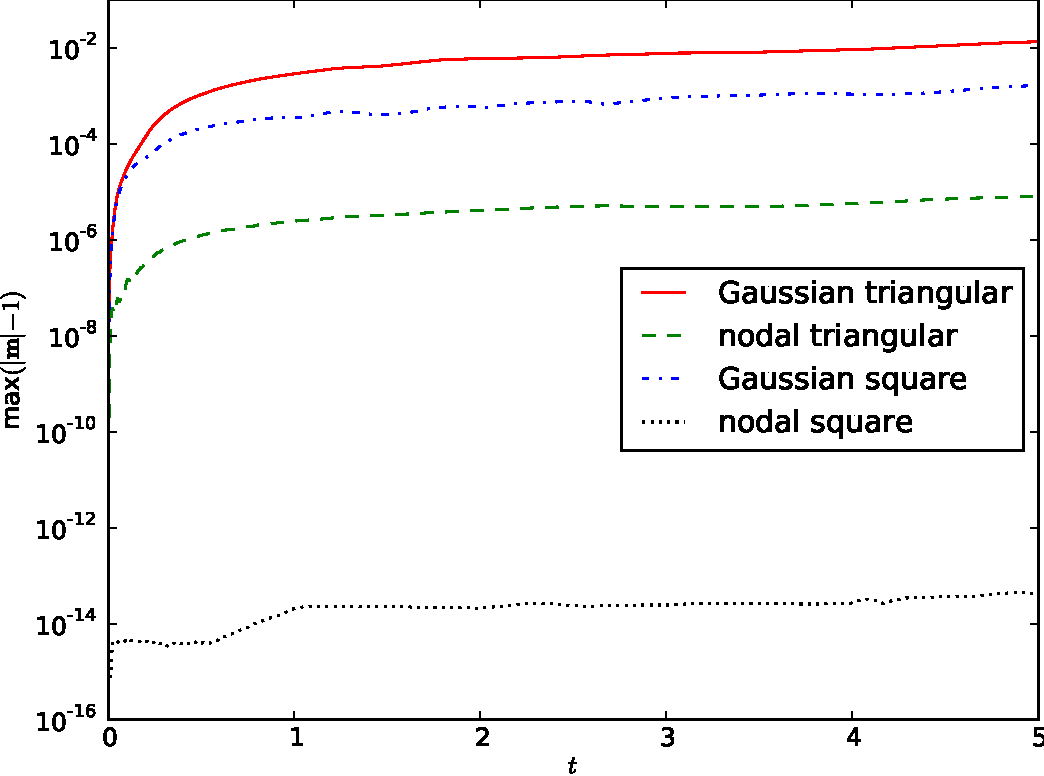
\includegraphics[width=0.8\textwidth]
  {plots/nonuniform-h-triangles-ml/mlengtherrormaxesvstimes.pdf}
  \caption{
    Evolution of $\myerr_{\abs{\mv}}$
    with various time integration schemes, quadratures, and element shapes
    for the 2D nonuniform field problem.
}
  \label{fig:ml-error-triangle-mesh}
\end{figure}

\begin{figure}
  \centering
  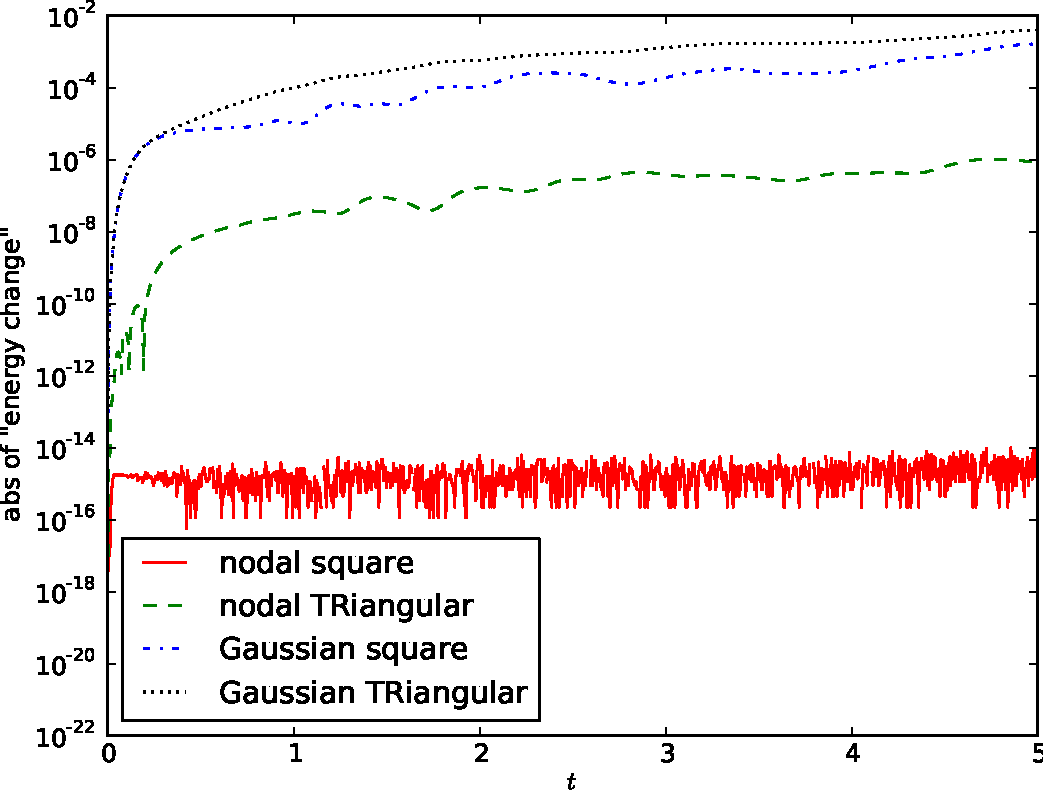
\includegraphics[width=0.8\textwidth]
  {plots/nonuniform-h-triangles-energy-error/absofenergychangevstimes.pdf}
  \caption{
    Evolution of the error in energy
    with various time integration schemes, quadratures, and element shapes
    for the undamped 2D nonuniform field problem.
  }
  \label{fig:energy-error-triangle-mesh}
\end{figure}

\subsection{Conclusions}

We have confirmed that the wave-like example is in some sense ``too easy'' and does not provide a rigorous test of geometric integration properties: IMR with Gaussian quadrature and TR do not conserve energy or $\abs{\mv}$ in general.

We have also shown an example problem where our implementation of IMR with nodal quadrature unexpectedly \emph{does not} conserve energy or $\abs{\mv}$ when used with a mesh of triangular elements.


% Don't allow floats from last section into this one
\FloatBarrier
\section{The \mumag standard problem \#4}

The \mumag standard problem \#4 \cite{mumag-website} is the benchmark problem most widely used to test implementations of dynamic micromagnetic models.
It involves modelling the reversal of an extremely thin cuboid film of permalloy-like material under two different applied fields.
Unfortunately FEM/BEM magnetostatic calcultations are ill-suited to thin film problems: the dense BEM matrix size is proportional to the number of nodes on the boundary and in a thin film every single node is on the boundary.
Additionally the key benefit of FEM/BEM (accurate resolution of complex geometries) is not required since the film is a simple cuboid.
However, since there are no other widely studied test problems and there are no problems with non-trivial magnetostatic and exchange effects for which an analytical solution is known, we use the standard problem to verify our implementation.


\subsection{Problem specification}

The magnetic domain is a sheet of magnetic material $500 \times 125 \times 3$nm with material parameters
\begin{equation}
  \begin{aligned}
    A &= 1.3\E{-11} \text{J/m}, \\
    M_s &= 8.0\E{5} \text{A/m}, \\
    \Kone &= 0.0, \\
    \gymagc &= 2.211 \E{5} \text{m/As}, \\
    \dampc &= 0.02.
  \end{aligned}
\end{equation}
The simulation is run with two different applied fields:
\begin{equation}
  \begin{aligned}
    \happ_1 = [-24.6, 4.3, 0.0] \E{-3}\text{A/m}, \\
    \happ_2 = [-35.5, -6.3, 0.0] \E{-3}\text{A/m}, \\
  \end{aligned}
  \label{eq:mumag-h-app}
\end{equation}
where we have converted from the magnetic flux intensity specified by the \mumag website to a magnetic field by dropping the factor of $\mu_0$.
The initial condition is the S-state given by slowly relaxing the magnetisation from the state created by a saturating field in the $[1,1,1]$ direction.

The magnetic parameters result in a magnetostatic exchange length (and unit length in our simulations) of
\begin{equation}
  l_{\text{ex}} = \sqrt{\frac{2A}{\mu_0 M_s^2}} = 5.6858\text{nm},
\end{equation}
hence the normalised dimensions are approximately $87.94 \times 21.98 \times 0.53$.
Our unit time is
\begin{equation}
  t_{\text{unit}} = \frac{1}{\gymagc M_s} = 5.653\text{ps}.
\end{equation}
The normalised applied fields are simply the fields given in \cref{eq:mumag-h-app} divided by $M_s = 8.0\E{5}$.


\subsection{Implementation details}

We use the FEM to spatially discretise the LLG equation and the Newton-Raphson method to solve the resulting non-linear systems as described in \cref{sec:galerk-meth-llg}.
The hybrid FEM/BEM method, described in \cref{sec:hybr-finit-elem}, is used for magnetostatic calculations.
For the coupling of LLG equation with the magnetostatic calculations we use both the monolithic and semi-implicit methods discussed in \cref{sec:solution-strategies}.
The solution of the monolithic linear system is done using the fully iterative preconditioner $\inexact{\precc}$, it turns out that for thin film problems the ILU(1) approximation to the LLG block, $\Fm$, is effective.
The decoupled systems resulting from the semi-implicit method are solved using the methods described in \cref{sec:llg-only-system}.

Both Gaussian quadrature and the nodal quadrature are used.
The TR, BDF2 and IMR adaptive time integration schemes (see \cref{sec:adapt-impl-midp,sec:aimr-implementation}) are tested.
Re-normalisation of the magnetisation is also tested for those schemes which do not naturally conserve $\abs{\mv}$.

As previously mentioned, the adaptive IMR requires an explicit time step for the estimation of the error.
This is implemented as described in \cref{sec:impl-deta}.
No coupling with the FEM/BEM calculations is required for this explicit step because only the value of the magnetostatic potential at the previous time step is required (which is already known from the IMR calculations of the previous step).

A structured mesh consisting of cuboid elements is used due to the simple geometry of the problem and the fact that we have observed issues with geometric integration on tetrahedral elements in \cref{sec:triangular-meshes}.
In the $z$ direction (out of the thin film plane) a single layer of elements is used at all refinements.
This is a standard approach, and is expected to give acceptable resolution because the exchange length of the material (the length scale over which the magnetisation can vary) is around twice the thickness.
The number of elements along the $x$ and $y$ axes, denoted $n_x$ and $n_y$, is varied but the ratio is fixed as $n_x = (500/125) n_y$ so that the element edge lengths in each direction are identical.
We use $n_x=75,100,125$, which gives edge lengths of 1.17, 0.89 and 0.70 exchange lengths respectively.

The Newton tolerance is fixed at $\ntol = 10^{-11}$, the adaptive integrator tolerance is $\toltt = 10^{-5}$ and the initial time step is $\dtx{0} = 10^{-4}$.
% We cap the time step at $\dtx{\text{max}} = 4.5$ to avoid issues with linear and solver converge at extremely large time steps.


To generate the initial S-state we run the simulation for 300 time units starting from the state $\mv=[1,1,1]$ with $\dampc = 1.0$ and the applied field
\begin{equation}
  \happ(t) =
  \begin{cases}
    10 (1- \frac{t}{100}) & t < 100, \\
    0 & t \geq 100.
  \end{cases}
\end{equation}
The time integrator history data is then set such that it has been in this state forever and the time step sizes are set to the initial value.
The relevant applied field as specified in the problem is then set and the simulation is continued.
The initial condition is always generated using the same numerical methods as are used in the simulation.

Note that with $\dampc = 1$ the time scale for the magnetisation to relax is much shorter than with $\dampc \sim 0.01$.
Hence the simulated time allowed for relaxation to the initial condition is sufficiently long to be considered ``slow'' despite the fact that it is much shorter than the simulated time for the dynamics calculations.


We compare our results against those submitted to the \mumag website by d'Aquino \etal \cite{mumag-website}.
These results were generated by a fixed time step monolithic IMR scheme with a finite difference spatial discretisation and the fast Fourier transform method for magnetostatic calculations \cite{DAquino2005}.



\subsection{General results}

For this problem we find that without either re-normalisation or geometric integration the time steps selected by the adaptive algorithms become unacceptably small (\ie the error becomes large).
Hence these cases were not run until completion and are not included in the results.

In \cref{fig:intial-mumag4} we show the initial S-state, as generated by IMR with nodal quadrature.
\begin{figure}
  \centering
  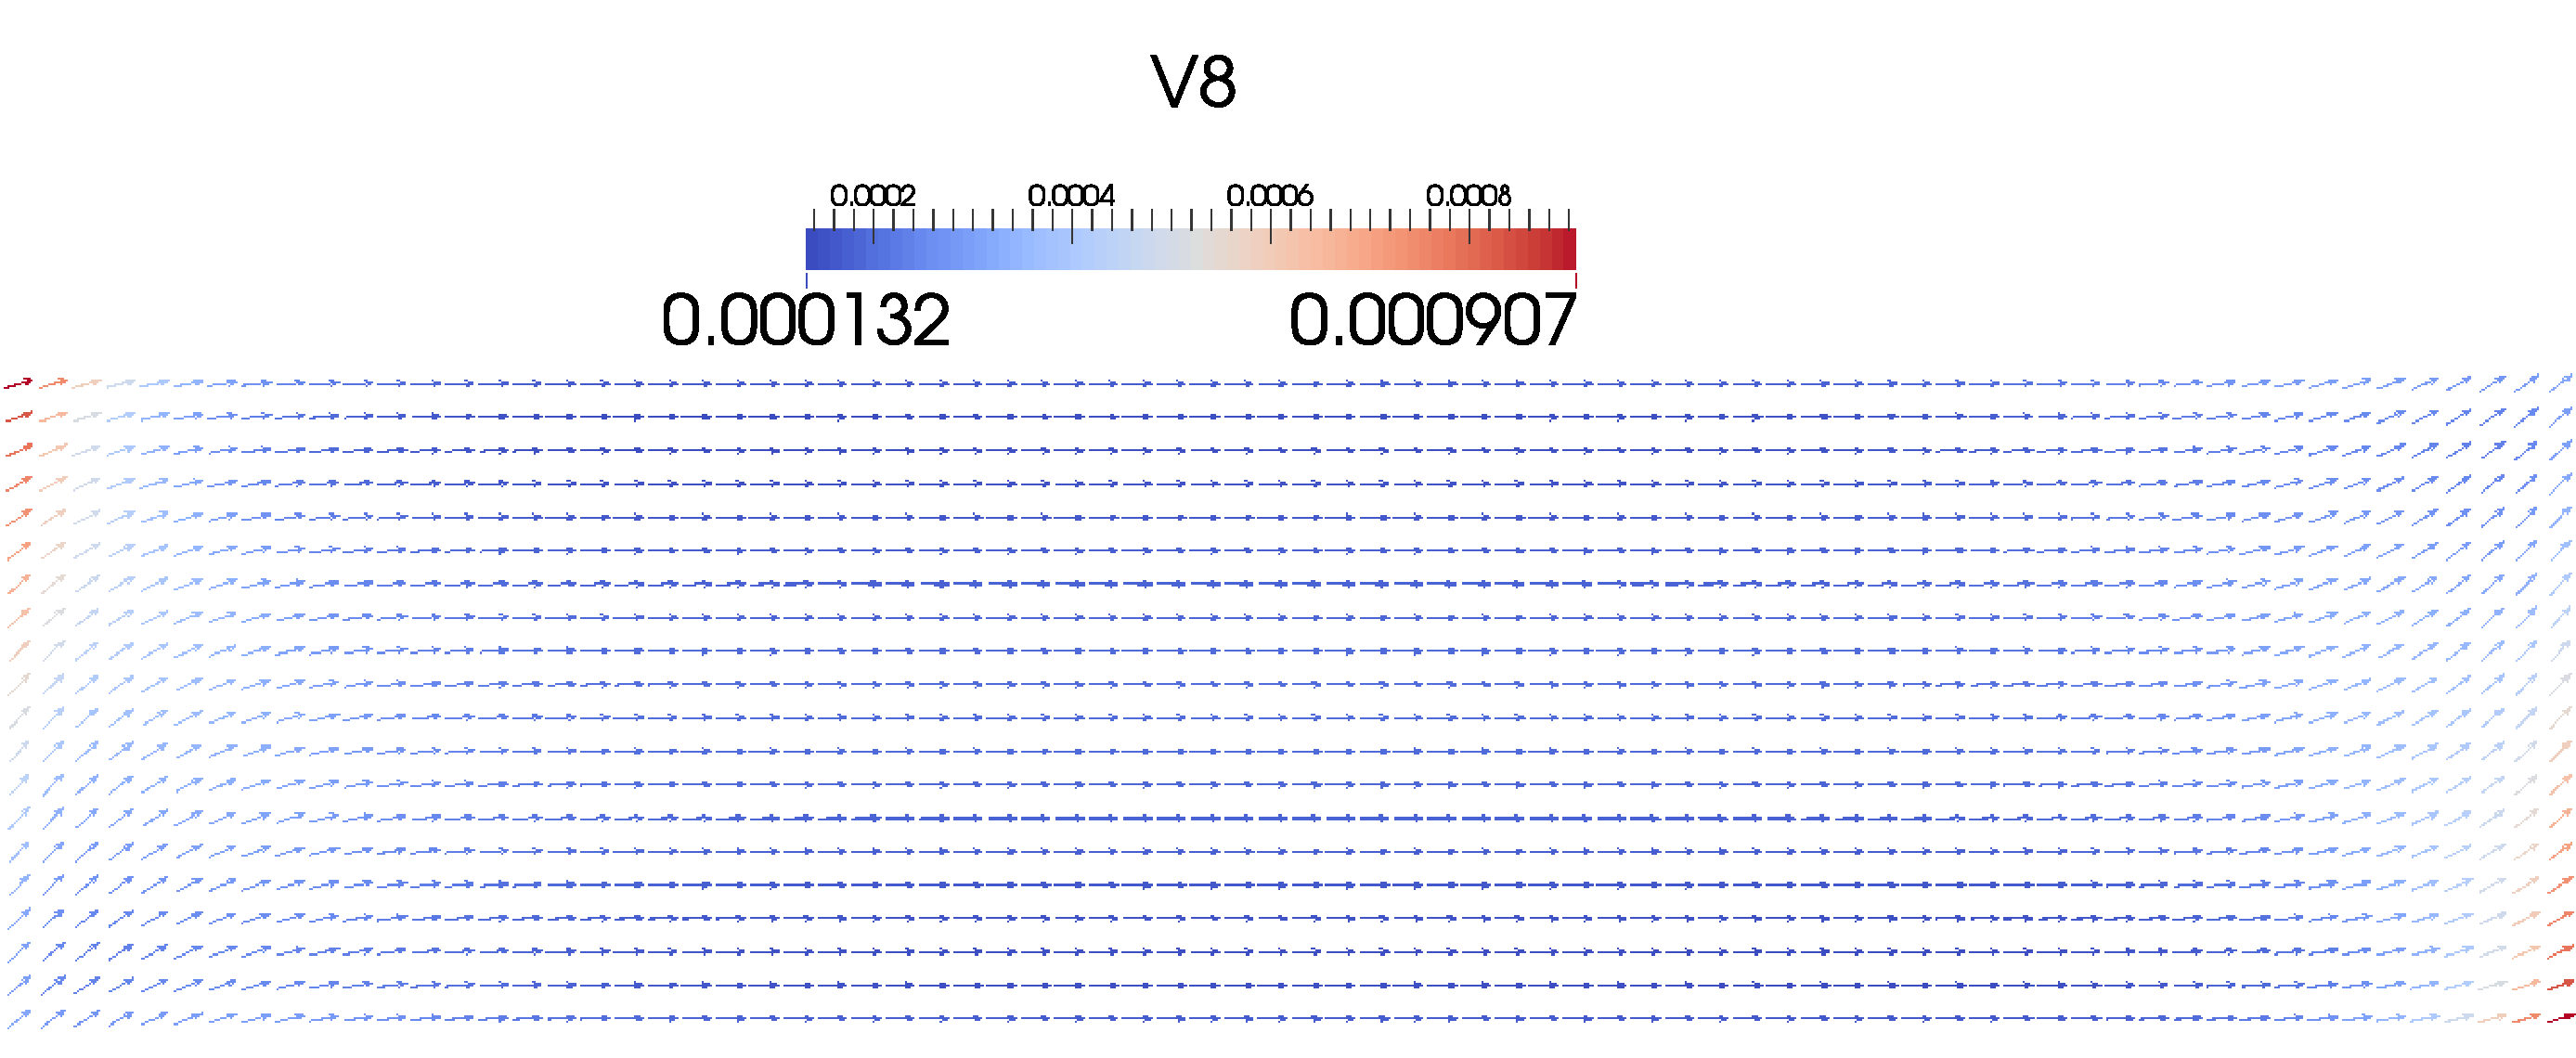
\includegraphics[width=0.8\textwidth]{images/mumag4-s-state.pdf}
  \caption{Initial S-state as generated by adaptive IMR with nodal quadrature and $n_x=75$ nodes along the $x$ direction.
    Colour indicates the $z$ (out of plane) component of magnetisation.
  }
  \label{fig:intial-mumag4}
\end{figure}

Next we show the mean magnetisation for the two fields from \cref{eq:mumag-h-app} in \cref{fig:nmag-comparison-mumag4-field1,fig:nmag-comparison-mumag4-field2} respectively.
Our results with smaller numbers of nodes, other time integration schemes, and smaller adaptive time integrator tolerance agree well with the results shown in \cref{fig:nmag-comparison-mumag4-field1,fig:nmag-comparison-mumag4-field2}.

The results agree reasonably well with the results obtained by d'Aquino except around $t=100$ when field 2 is used.
We have also tested the behaviour when using IMR with fixed time steps or alternative methods for generating the initial S-state but these have no effect on our results.
However, it is worth noting that all of the submitted solutions on the \mumag website \cite{mumag-website} behave differently for this part of the problem!
The issues may be due to corner singularities in the magnetostatic field and, if so, could be resolved by the use of higher order solution and test basis functions for the magnetostatic potential \cite{Schrefl1997}.


The same plots show the time step selection behaviour.
During relaxation (negative time in the figures) the time step has a large value initially, which decreases as the field decreases and the relaxation happens, then very large once the field becomes zero.
During the dynamics(positive time in the figures): a reasonable large time step is selected initially.
It then decreases around the time of the peak in $\mv$ and steadily increases as the oscillations are damped out.
The behaviour observed for the second field is essentially the same.

\begin{figure}
  \centering
  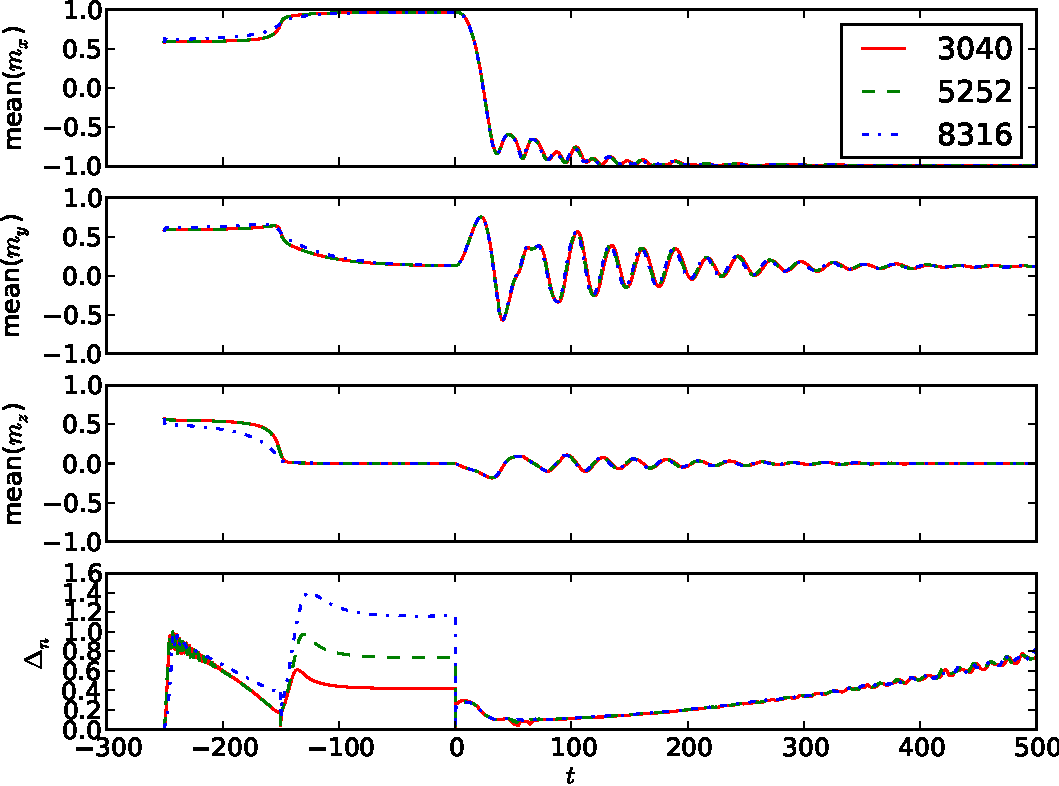
\includegraphics[width=0.8\textwidth]{plots/mumag4_convergence/mumag4_field1-meanmxsvs-meanmysvs-meanmzsvs-dtsvstimes.pdf}
  \caption{
    Evolution of the mean magnetisation for the \mumag problem \#4 with field 1 using monolithic IMR with nodal quadrature.
    For comparison we also show the results submitted to the \mumag website by d'Aquino \etal \cite{mumag-website}.
}
  \label{fig:nmag-comparison-mumag4-field1}
\end{figure}

\begin{figure}
  \centering
  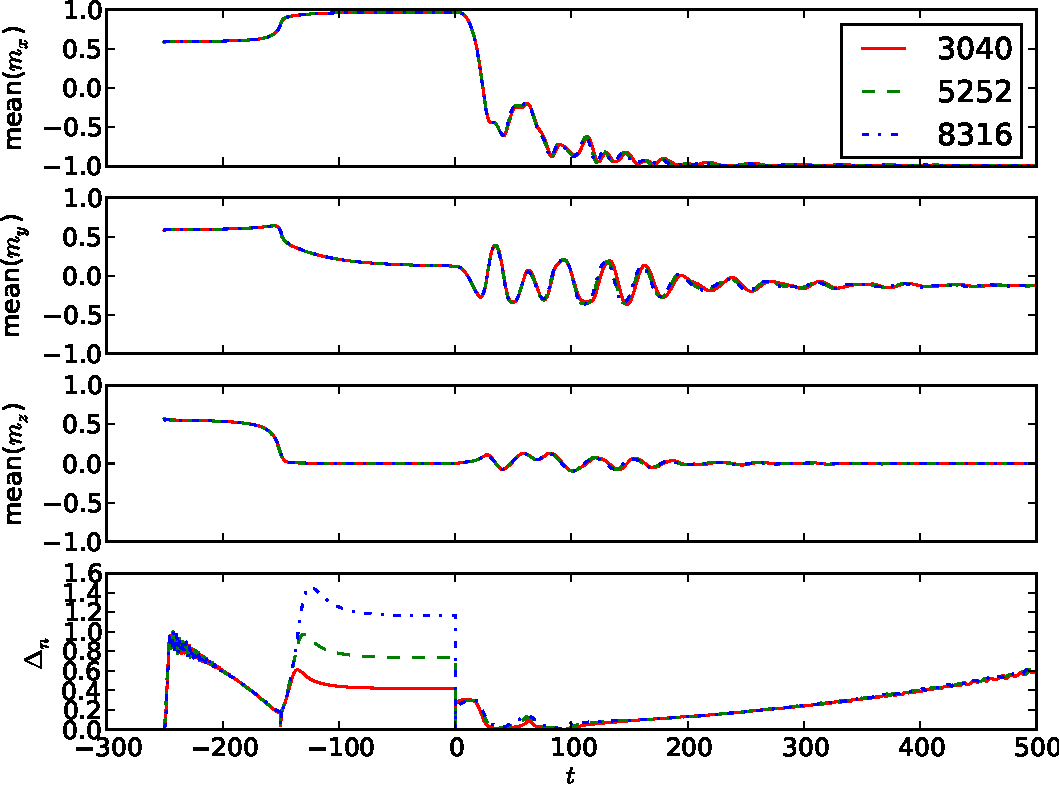
\includegraphics[width=0.8\textwidth]{plots/mumag4_convergence/mumag4_field2-meanmxsvs-meanmysvs-meanmzsvs-dtsvstimes.pdf}
  \caption{
    Evolution of the mean magnetisation for the \mumag problem \#4 with field 2 using monolithic IMR with nodal quadrature.
    For comparison we also show the results submitted to the \mumag website by d'Aquino \etal \cite{mumag-website}.
  }
  \label{fig:nmag-comparison-mumag4-field2}
\end{figure}


%
% Also the state of the system at the time when $m_x$ crosses zero for field 2 is shown in \cref{fig:mumag4-spatial-x-crossing-0}.

% \begin{figure}
%   \centering
%   
\includegraphics[width=0.8\textwidth]{images/placeholder}
%   \caption{The state of the system at the time when $m_x$ crosses zero}
%   \label{fig:mumag4-spatial-x-crossing-0}
% \end{figure}


We show a comparison of the magnetisation generated using IMR with nodal quadrature and monolithic or decoupled approach in \cref{fig:mumag4-implicit-decoupled}.
The dynamics are very similar, but the monolithic method is able to take larger time steps and has less noise in the size step during the initial relaxation.
\begin{figure}
  \centering
  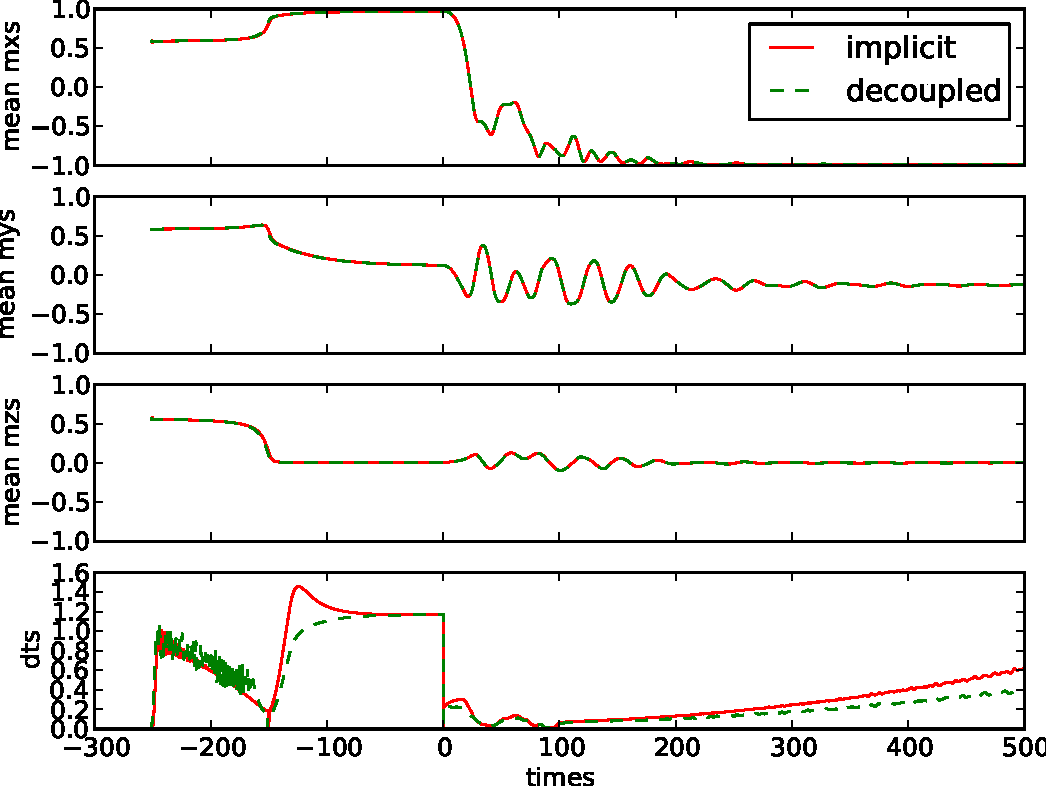
\includegraphics[width=0.8\textwidth]
  {plots/monolithic_vs_decoupled/meanmxsvs-meanmysvs-meanmzsvs-dtsvstimes.pdf}
  \caption{
    Evolution of the mean magnetisation for the \mumag problem \#4 with field 2 using IMR with nodal quadrature and monolithic (implicit) or semi-implicit (decoupled) coupling to the magnetostatics problem.
  }
  \label{fig:mumag4-implicit-decoupled}
\end{figure}

\subsection{Geometric integration properties}

The evolution of the maximum nodal error in the magnetisation length for the decoupled and implicit methods is shown in \cref{fig:imr-conservation}.
As expected both coupling approaches conserve $\abs{\mv}$ to around the Newton tolerance.
\begin{figure}
  \centering
  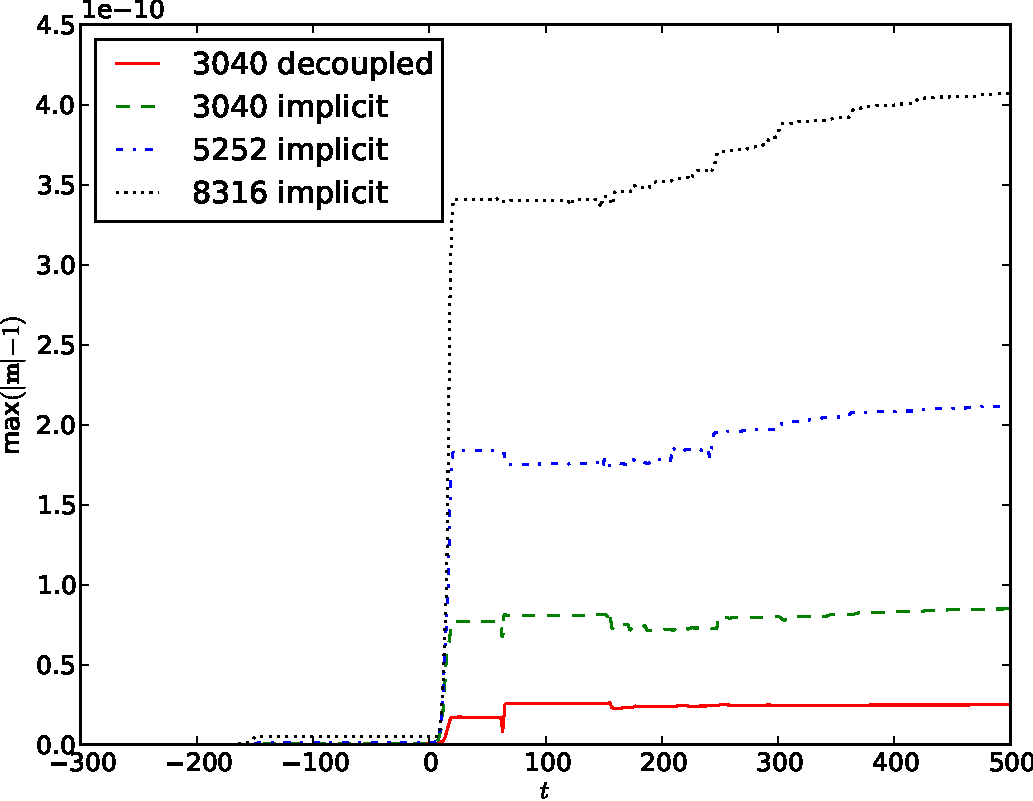
\includegraphics[width=0.8\textwidth]{plots/mumag4_ml/mlengtherrormaxesvstimes.pdf}
  \caption{
    Evolution of $\myerr_{\abs{\mv}}$
    with IMR, nodal quadrature and both coupling strategies
    for the \mumag problem \#4 with field 2.
  }
  \label{fig:imr-conservation}
\end{figure}


The evolution of the energy of the system when $\dampc = 0$ is shown in \cref{fig:energy-conservation}.
It can be seen that neither the monolithic or decoupled methods give the desired conservation behaviour.
From various other experiments we have drawn the conclusion that this occurs when the magnetostatic calculations are introduced.
We believe the cause is the use of a collocation rather than a Galerkin approach to the discretisation of the boundary element part of the magnetostatic calculation.
Collocation based approaches do not preserve the symmetry of the underlying operators, and so would be expected to cause issues with energy conservation based on \cref{eqn:imr-linop} and \cref{eq:orth-energy}.
Implementation of a Galerkin BEM within the \oomph framework, in order to test this theory, is ongoing.

\begin{figure}
  \centering
  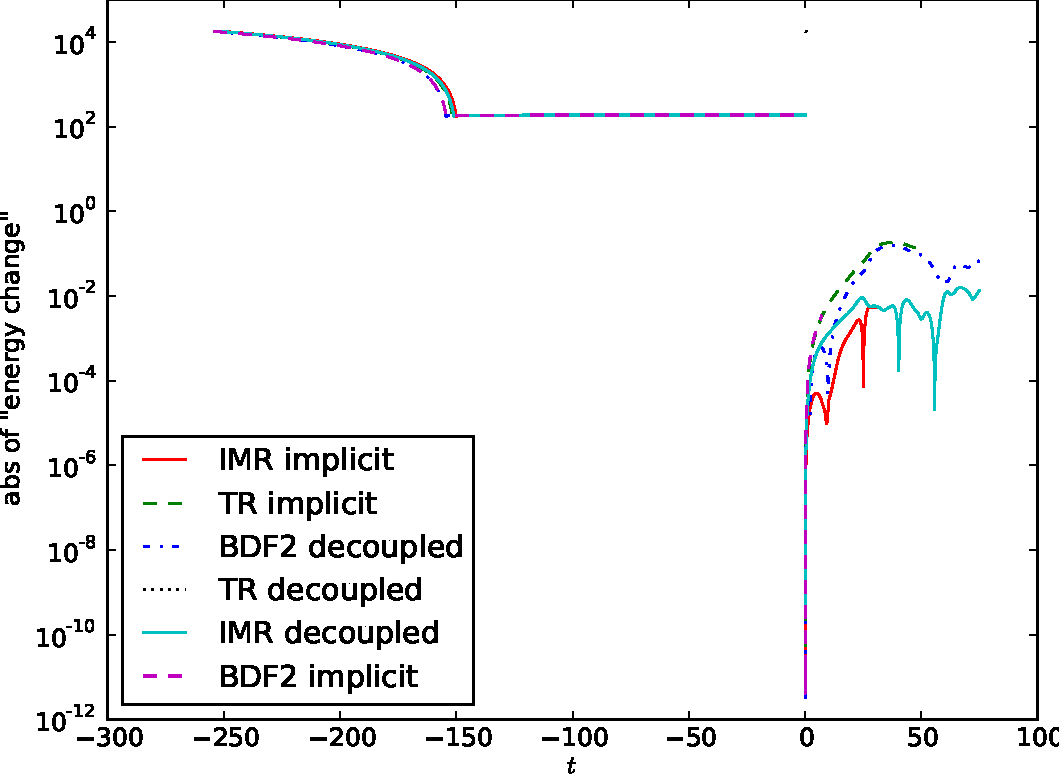
\includegraphics[width=0.8\textwidth]
  {plots/sq_mumag4_energy_conservation/absofenergychangevstimes.pdf}
  \caption{
    Evolution of the error in energy
    with various time integration schemes, quadratures, and coupling strategies
    for the undamped \mumag problem \#4 with field 2.
    Results for other combinations of methods are very similar.
  }
  \label{fig:energy-conservation}
\end{figure}


\subsection{Effectiveness of the linear and non-linear solver}

Here we examine the effectiveness of the iterative linear solver for the monolithic method introduced in \cref{sec:fully-implicit-bem} for the standard problem.
The number of iterations required for convergence as the number of nodes varys are shown in \cref{fig:mumag4-solver-iterations}.
Note that while they increase with the number of nodes, $\Nn$, they remain reasonable for the problem sizes required good accuracy in this example.
The time taken to set up the preconditioner is displayed in \cref{fig:mumag4-solver-time}, again it grows with the number of nodes but remains reasonable for all cases shown here.
Also note that with nodal quadrature the preconditioner is cheaper to set up but less effective, to counteract this a higher level of fill-in could be used with nodal quadrature.

\begin{figure}
  \centering
  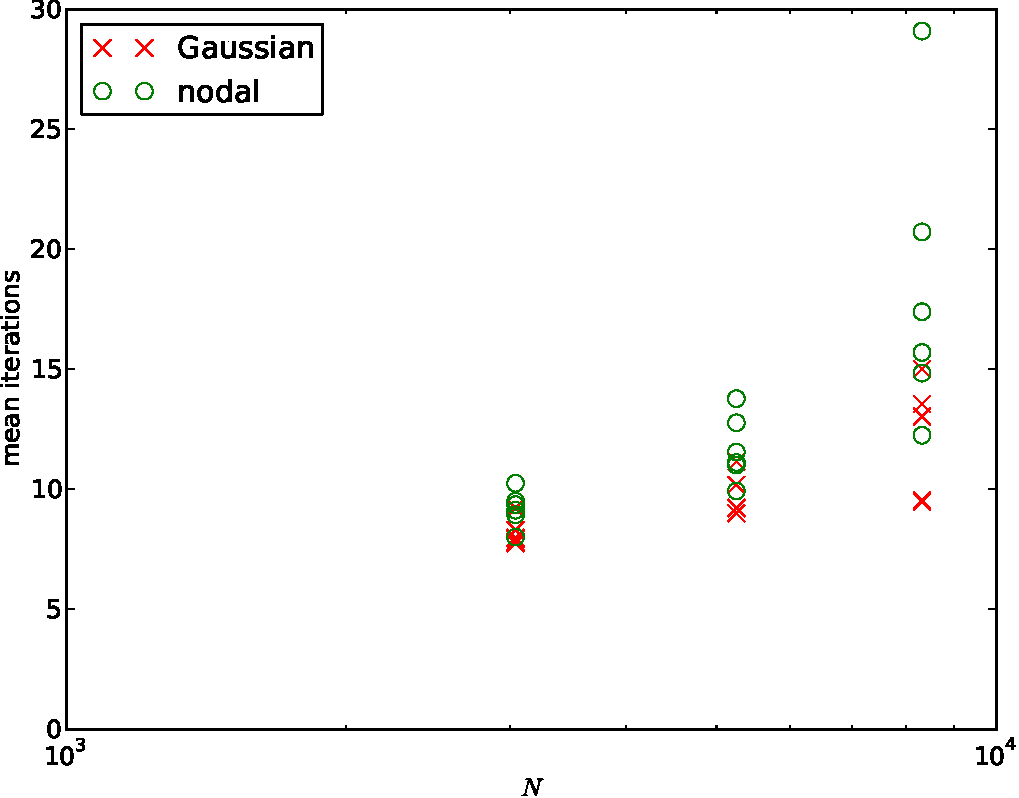
\includegraphics[width=0.8\textwidth]
  {plots/mumag4_monolithic_its/meanofnsolveritersvsinitialnnode.pdf}
  \caption{
    GMRES iterations to converge against problem size for the monolithic system using the inexact preconditioner $\inexact{\precc}$ with the various time integration schemes, quadratures, and applied fields for the \mumag problem \#4 (including the calculation of the relaxed initial condition).
}
  \label{fig:mumag4-solver-iterations}
\end{figure}

\begin{figure}
  \centering
  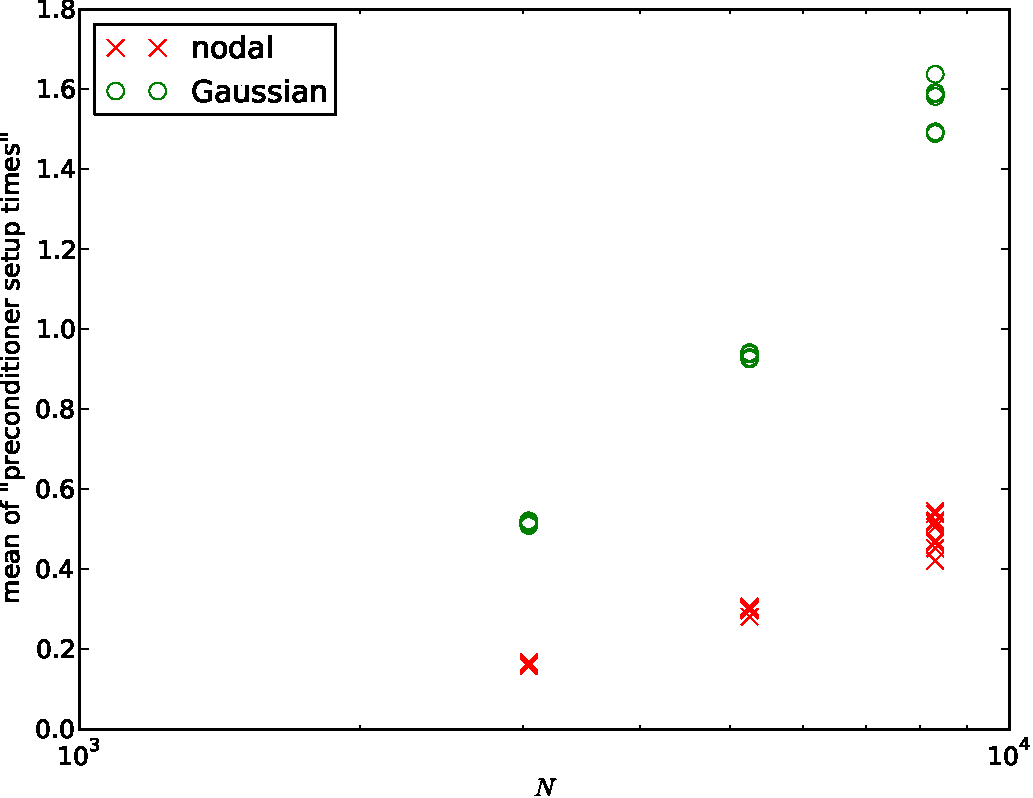
\includegraphics[width=0.8\textwidth]
  {plots/mumag4_monolithic_its/meanofpreconditionersetuptimesvsinitialnnode.pdf}
  \caption{
    Time in seconds to set up the inexact preconditioner $\inexact{\precc}$
    against problem size for the monolithic system using the inexact preconditioner $\inexact{\precc}$
    with the various time integration schemes, quadratures, and applied fields
    for the \mumag problem \#4 (including the calculation of the relaxed initial condition).
  }
  \label{fig:mumag4-solver-time}
\end{figure}


Next we look at the number of iterations of the Newton-Raphson method required to solve the monolithically coupled non-linear system.
The mean number of iterations required for convergence is consistently just over 2 (and always less than 3) despite the extremely tight tolerance and the very large time steps used in the calculation of the initial condition.
In particular we note that the number of iterations required is significantly lower than the $\sim 14$ quasi-Newton iterations required for the monolithic method used in \cite{DAquino2005}.
The various other problems covered in this chapter required similar numbers of Newton-Raphson iterations.

\begin{figure}
  \centering
  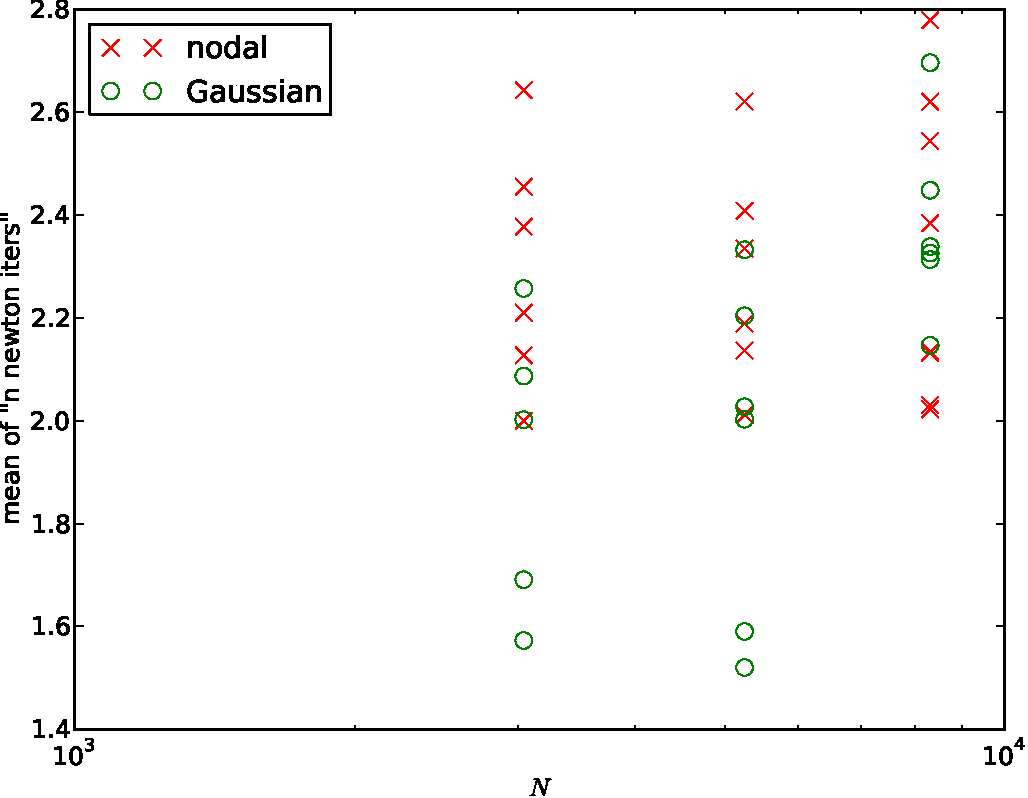
\includegraphics[width=0.8\textwidth]
  {plots/mumag4_monolithic_its/meanofnnewtonitersvsinitialnnode.pdf}
  \caption{Newton-Raphson iterations to converge against problem size
    for the monolithic system with the various time integration schemes, quadratures, and applied fields for the \mumag problem \#4 (including the calculation of the relaxed initial condition).}
  \label{fig:mumag4-newton-iters}
\end{figure}


We do not explore the total solve times of the various methods for this example:
due to the fact that we have not used a hierarchical matrix representation of the dense block and the extremely large number of boundary nodes the solve times are dominated by the calculations involving the BEM matrix.
Hence any timing results would be meaningless for practical problems in which the FEM/BEM method is appropriate.


\subsection{Conclusions}

Our methods give results for the \mumag problem \#4 which converge well and match up reasonably well with the results of other models.

We observe the expected conservation of magnetisation length with IMR and nodal quadrature.
However, we do not observe the expected conservation of energy.
We believe that this is due to the use of a collocation approach for the discretisation of the BEM part of the problem.
Collocation approaches do not preserve symmetry of underlying operators and so the symmetry of the effective field operator, which is essential for the energy properties of IMR, will have been lost.
Implementation of a Galerkin BEM method is ongoing, but there are no theoretical difficulties (see \eg \cite[58]{Borm2003}).

Finally we have shown that, aside from issues with the lack of a hierarchical matrix implementation for rectangular boundary elements, we can efficiently solve the monolithic non-linear problem resulting from coupling the LLG with FEM/BEM magnetostatics calculations.
Application of Newton-Raphson method results in around 2.2 Newton iterations per non-linear.
The use of GMRES preconditioned by $\inexact{\precc}$ results in around 15 Krylov iterations per linear solve, with a reasonable setup time.



\section{Conclusions}

In this chapter we have demonstrated the effectiveness of the methods developed in the rest of this thesis.

We observed that our adaptive IMR algorithm selects appropriate time steps even for complex problems involving exchange and magnetostatics.
We have shown that IMR with nodal quadrature retains its magnetisation length conservation property on a number of problems, but that it fails on certain meshes of triangular elements.
Similarly IMR (with nodal quadrature) provides energy conservation for problems without FEM/BEM magnetostatics, but that the energy conservation fails when collocation FEM/BEM magnetostatics calculations are included.

Our methods converge exactly as expected to an exact solution of the LLG with exchange effective field.
Their accuracy on the first applied field of the \mumag standard problem \#4 also appears to be very good.
For the second field the results agree well with a finite difference based method using a similar time integration scheme only up to $t=100$, but all of the solutions submitted to the \mumag website disagree around this time.


%%% Local Variables:
%%% mode: latex
%%% TeX-master: "main"
%%% End:
